\sloppy
\documentclass[12pt,a4paper]{report}

% ================== PACKAGES ==================
\usepackage[utf8]{inputenc}
\usepackage[T1]{fontenc}
\usepackage[french]{babel}
\usepackage[a4paper,top=2.5cm,bottom=2.5cm,left=2.5cm,right=2.5cm]{geometry}
\usepackage{setspace}
\usepackage{graphicx}
\usepackage{xcolor}
\usepackage{ragged2e}
\usepackage{hyperref}
\usepackage{titlesec}
\usepackage{tocloft}
\usepackage{fancyhdr}
\usepackage{caption}
\usepackage{float}
\usepackage{amsmath, amsfonts, amssymb}
\usepackage{tikz}
\usepackage{atbegshi}
\usepackage{tcolorbox}
\usepackage{booktabs}
\usepackage{array}
\usepackage{enumitem}
\usepackage{listings}
\usepackage{tabularx}
\usepackage{colortbl}
\usepackage{pifont}
\usetikzlibrary{shapes.geometric,arrows.meta,positioning,fit,backgrounds,
                decorations.pathreplacing,shadows.blur,calc}

% ================== COULEURS ==================
\definecolor{bleuUniv}{RGB}{0,60,130}
\definecolor{bleuClair}{RGB}{0,102,204}
\definecolor{bleuPale}{RGB}{220,232,248}
\definecolor{bleuMoyen}{RGB}{0,80,160}
\definecolor{bleuTresClair}{RGB}{240,245,255}
\definecolor{grisClair}{RGB}{248,249,252}
\definecolor{grisChap}{RGB}{90,90,100}
\definecolor{blanc}{RGB}{255,255,255}

% ================== CONFIGURATION ==================
\setcounter{secnumdepth}{3}
\setcounter{tocdepth}{3}

\hypersetup{
    colorlinks=true,
    linkcolor=bleuUniv,
    urlcolor=bleuMoyen,
    citecolor=bleuUniv,
    pdfauthor={Die Mbaye, Mouhamad Al Amine Ba},
    pdftitle={Jokko Agro : une plateforme blockchain-IA pour la certification et la monétisation des produits agricoles},
    pdfsubject={De la reconnaissance vocale Wolof à la certification on-chain : un écosystème numérique complet pour l'agriculture sénégalaise}
}

\setstretch{1.25}
\graphicspath{{images/}}

% ================== TCOLORBOX STYLES ==================
\tcbuselibrary{skins,breakable}
\tcbset{
  chapterbox/.style={
    enhanced,
    colback=bleuTresClair,
    colframe=bleuUniv,
    boxrule=1.2mm,
    arc=5mm,
    fonttitle=\bfseries\Large\color{white},
    colbacktitle=bleuUniv,
    attach boxed title to top center={yshift=-3mm},
    boxed title style={arc=3mm, colback=bleuUniv},
    top=6mm,
    width=\textwidth
  },
  infobox/.style={
    enhanced,
    colback=bleuTresClair,
    colframe=bleuUniv,
    boxrule=0.8mm,
    arc=4mm,
    fonttitle=\bfseries\color{white},
    colbacktitle=bleuMoyen,
    attach boxed title to top left={yshift=-2mm,xshift=6mm},
    boxed title style={arc=2mm},
    width=\textwidth
  },
  definbox/.style={
    enhanced,
    colback=white,
    colframe=bleuUniv,
    boxrule=1pt,
    arc=3mm,
    left=4mm,
    borderline west={3pt}{0pt}{bleuUniv},
    width=\textwidth
  },
  synthbox/.style={
    enhanced,
    colback=bleuUniv,
    colframe=bleuUniv,
    coltext=white,
    boxrule=0pt,
    arc=5mm,
    fonttitle=\bfseries\Large\color{white},
    center title,
    width=\textwidth
  },
  tablebox/.style={
    enhanced,
    colback=white,
    colframe=bleuUniv,
    boxrule=0.8mm,
    arc=3mm,
    width=\textwidth
  }
}

% ================== STYLE DES CHAPITRES ==================
\titleformat{\chapter}[display]
  {\normalfont}
  {%
    \begin{tikzpicture}[remember picture]
      \fill[bleuUniv] (0,0) rectangle (\textwidth,1.8cm);
      \fill[bleuMoyen] (0,0) rectangle (\textwidth,0.22cm);
      \node[anchor=west, white, font=\Large\bfseries\scshape,
            inner sep=0pt] at (0.5cm,1.0cm)
        {\chaptertitlename\ \thechapter};
      \node[anchor=east, white!60, font=\small\itshape,
            inner sep=0pt] at (\textwidth-0.4cm,1.0cm)
        {Jokko Agro};
    \end{tikzpicture}%
  }
  {0pt}
  {%
    \vspace{0.2cm}
    \color{bleuUniv}\huge\bfseries
  }
  [\vspace{4pt}{\color{bleuUniv}\titlerule[1.5pt]}\vspace{6pt}]

\titleformat{name=\chapter,numberless}[display]
  {\normalfont}
  {%
    \begin{tikzpicture}
      \fill[bleuUniv] (0,0) rectangle (\textwidth,1.8cm);
      \fill[bleuMoyen] (0,0) rectangle (\textwidth,0.22cm);
    \end{tikzpicture}%
  }
  {0pt}
  {\color{bleuUniv}\huge\bfseries}
  [\vspace{4pt}{\color{bleuUniv}\titlerule[1.5pt]}\vspace{6pt}]

\titlespacing*{\chapter}{0pt}{-50pt}{20pt}

\titleformat{\section}{\large\bfseries\color{bleuUniv}}{\thesection}{1em}{}
  [{\color{bleuClair}\titlerule[0.8pt]}]
\titleformat{\subsection}{\normalsize\bfseries\color{bleuMoyen}}{\thesubsection}{1em}{}
\titleformat{\subsubsection}{\normalsize\bfseries\color{grisChap}}{\thesubsubsection}{1em}{}

\titlespacing*{\section}{0pt}{12pt}{5pt}
\titlespacing*{\subsection}{0pt}{8pt}{3pt}
% ================== DOUBLE CADRE ==================
% Définir une bordure sur toutes les pages
\AtBeginShipout{\AtBeginShipoutAddToBox{%
  \begin{tikzpicture}[remember picture,overlay,inner sep=0,outer sep=0]
    % Bordure extérieure
    \draw[blue!70!black, line width=2pt]
      ([xshift=-0.8cm, yshift=-0.8cm]current page.north east) --
      ([xshift=0.8cm, yshift=-0.8cm]current page.north west) --
      ([xshift=0.8cm, yshift=0.8cm]current page.south west) --
      ([xshift=-0.8cm, yshift=0.8cm]current page.south east) -- cycle;

    % Bordure intérieure (1er niveau)
    \draw[black!50, thin]
      ([xshift=-1.1cm, yshift=-0.5cm]current page.north east) --
      ([xshift=1.1cm, yshift=-0.5cm]current page.north west) --
      ([xshift=1.1cm, yshift=0.5cm]current page.south west) --
      ([xshift=-1.1cm, yshift=0.5cm]current page.south east) -- cycle;

    % Bordure intérieure (2e niveau)
    \draw[black!30, black]
      ([xshift=-0.5cm, yshift=-1.1cm]current page.north east) --
      ([xshift=0.5cm, yshift=-1.1cm]current page.north west) --
      ([xshift=0.5cm, yshift=1.1cm]current page.south west) --
      ([xshift=-0.5cm, yshift=1.1cm]current page.south east) -- cycle;
  \end{tikzpicture}%
}}


% ================== EN-TÊTE / PIED DE PAGE ==================
\pagestyle{fancy}
\fancyhf{}
\fancyhead[L]{\small\color{bleuUniv}\textit{Jokko Agro --- Plateforme d'Agriculture Intelligente}}
\fancyhead[R]{\small\color{bleuUniv}\textit{UCAD --- Licence 3 TDSI}}
\fancyfoot[C]{\small\color{bleuUniv}\thepage}
\renewcommand{\headrulewidth}{0.6pt}
\renewcommand{\headrule}{\color{bleuUniv}\hrule width\headwidth height 0.6pt}
\setlength{\headheight}{15pt}

% ================== STYLE DE LA TABLE DES MATIÈRES ==================
\renewcommand{\contentsname}{Table des Matières}
\setlength{\cftbeforetoctitleskip}{0.3cm}
\setlength{\cftaftertoctitleskip}{1cm}
\renewcommand{\cftchapfont}{\bfseries\large\color{bleuUniv}}
\renewcommand{\cftchappagefont}{\bfseries\large\color{bleuUniv}}
\setlength{\cftchapnumwidth}{2.8em}
\setlength{\cftchapindent}{0em}
\renewcommand{\cftchapleader}{\color{bleuUniv}\cftdotfill{\cftdotsep}}
\renewcommand{\cftsecfont}{\normalsize\color{black}}
\renewcommand{\cftsecpagefont}{\normalsize\color{bleuUniv}}
\setlength{\cftsecindent}{2.8em}
\setlength{\cftsecnumwidth}{2.5em}
\renewcommand{\cftsecleader}{\color{bleuUniv!50}\cftdotfill{\cftdotsep}}
\renewcommand{\cftsubsecfont}{\small\color{grisChap}}
\setlength{\cftsubsecindent}{5.8em}
\setlength{\cftparskip}{0.18cm}
\setlength{\cftbeforechapskip}{0.3cm}
\renewcommand{\cftdot}{.}
\renewcommand{\cftdotsep}{2}

% ================== STYLE DE LA TABLE DES FIGURES ==================
\renewcommand{\listfigurename}{Table des Figures}
\setlength{\cftbeforeloftitleskip}{0.3cm}
\setlength{\cftafterloftitleskip}{0.5cm}
\renewcommand{\cftfigfont}{\normalsize\color{black}}
\renewcommand{\cftfigpagefont}{\normalsize\color{bleuUniv}}
\renewcommand{\cftfigleader}{\color{bleuUniv!50}\cftdotfill{\cftdotsep}}

% ================== STYLE DE LA LISTE DES ABRÉVIATIONS ==================

% ================== LISTINGS ==================
\lstset{
  basicstyle=\footnotesize\ttfamily,
  backgroundcolor=\color{grisClair},
  frame=single,
  rulecolor=\color{bleuUniv!40},
  breaklines=true,
  keywordstyle=\bfseries\color{bleuUniv},
  commentstyle=\itshape\color{grisChap},
  stringstyle=\color{bleuMoyen},
  numbers=left,
  numberstyle=\tiny\color{grisChap},
  xleftmargin=15pt,
  tabsize=2
}

% ================== DÉBUT DOCUMENT ==================
\begin{document}
\pagestyle{empty}
\thispagestyle{empty}

% =========================================================
%                      PAGE DE GARDE
% =========================================================
\begin{titlepage}
\thispagestyle{empty}

\begin{minipage}{0.45\textwidth}
\raggedright

\includegraphics[height=2.6cm]{images/logo-ucad.png}
\end{minipage}
\hfill
\begin{minipage}{0.45\textwidth}
\raggedleft

\includegraphics[height=2.6cm]{images/logo-lacgaa.jpeg}
\end{minipage}

\vspace{0.8cm}

\begin{minipage}{0.48\textwidth}
\raggedright
{\color{bleuUniv}\small
Université Cheikh Anta Diop de Dakar\\
Faculté des Sciences et Techniques\\
Département Mathématiques et Informatique
}
\end{minipage}
\hfill
\begin{minipage}{0.48\textwidth}
\raggedleft
{\color{bleuUniv}\small
Laboratoire d'Algèbre, de Cryptographie,\\
de Géométrie Algébrique et Applications\\
\textbf{LACGAA}
}
\end{minipage}

\vspace{1cm}

\begin{center}
{\normalsize\bfseries Licence 3 --- Transmission de Données et Sécurité de l'Information}
\end{center}

\vspace{1.5cm}

% ================== TITRE STYLISÉ ==================
\begin{center}
\begin{tikzpicture}
\node[inner sep=0pt] (box) {
  \begin{minipage}{0.85\textwidth}
  \centering
  \vspace{0.5cm}

  % Titre principal avec effet de shadow
  {\fontsize{28}{32}\selectfont\bfseries\color{bleuUniv}
  JOKKO AGRO}\\[0.3cm]

  % Ligne décorative
  \begin{tikzpicture}
  \draw[bleuClair, line width=0.8pt] (0,0) -- (6,0);
  \end{tikzpicture}
  \vspace{0.3cm}

  % Sous-titre avec style élégant
  {\fontsize{16}{20}\selectfont\scshape\color{bleuMoyen}
  une plateforme blockchain-IA pour\\[0.2cm]
  la certification et la monétisation\\[0.2cm]
  des produits agricoles}

  \vspace{0.5cm}
  \end{minipage}
};
\draw[line width=1.2pt,color=bleuUniv](box.north west) rectangle (box.south east);
\draw[line width=2.8pt,color=bleuUniv](box.south west)--(box.south east);
\end{tikzpicture}
\end{center}

\vspace{1.2cm}

\begin{minipage}{0.45\textwidth}
\raggedright
{\normalsize Présenté et soutenu par :\\[0.3cm]
\textcolor{bleuUniv}{\textbf{ Die Mbaye}}\\
\textcolor{bleuUniv}{\textbf{Mouhamad Al Amine Ba}}
}
\end{minipage}
\hfill
\begin{minipage}{0.45\textwidth}
\raggedleft
{\normalsize Sous la direction de :\\[0.3cm]
\textcolor{bleuUniv}{\textbf{Mme Ba Aminata}}
}
\end{minipage}

\vspace{1.2cm}

\begin{center}
\fcolorbox{bleuUniv}{white}{
\begin{minipage}{0.85\textwidth}
\vspace{0.3cm}\centering
{\Large\bfseries\color{bleuUniv}Jury}\\[0.4cm]
\begin{tabular}{p{7cm} p{4cm}}
\textcolor{bleuUniv}{Président : Dr Aminata Ngome BA} & \textcolor{bleuUniv}{UCAD}\\[0.3cm]
\textcolor{bleuUniv}{Membres : Mme Nafy Dione} & \textcolor{bleuUniv}{UCAD}\\
\textcolor{bleuUniv}{\hspace{1cm}M. Habib Ndiaye} & \textcolor{bleuUniv}{UCAD}\\
\textcolor{bleuUniv}{\hspace{1cm}M. Ndiagua} & \textcolor{bleuUniv}{UCAD}
\end{tabular}
\vspace{0.3cm}
\end{minipage}
}
\end{center}

\vfill

\begin{center}
{\normalsize\bfseries Année académique 2024--2025}
\end{center}
\end{titlepage}

% =========================================================
%           DÉDICACES & REMERCIEMENTS
% =========================================================
\clearpage\thispagestyle{empty}
\vspace*{-1.5cm}
\begin{center}{\Huge\bfseries Dédicaces \& Remerciements}\end{center}
\vspace{0.1cm}\hrule\vspace{0.1cm}
\begin{center}
\includegraphics[width=0.30\textwidth]{images/Dedicace.png}\end{center}
\vspace{0.1cm}
{\Large\itshape Bismillahi Rahmani Rahim, au nom de Dieu le Tout Miséricordieux, le Très Miséricordieux.}
\vspace{0.35cm}

{\Large Nous dédions ce mémoire :}
\vspace{0.2cm}
{\large
\begin{itemize}
  \item[$\star$] À nos très chers \textcolor{bleuUniv}{parents}. Puisse Allah nous protéger, vous accorder santé, bonheur et longue vie, et fasse en sorte que nous ne vous décevions jamais.
  \item[$\star$] À nos chers \textcolor{bleuUniv}{frères et sœurs}. Puisse Allah vous garder, éclairer votre route et vous aider à réaliser vos rêves les plus chers.
  \item[$\star$] À nos \textcolor{bleuUniv}{oncles et tantes}. Que le Tout-Puissant vous accorde une longue vie.
  \item[$\star$] À nos \textcolor{bleuUniv}{amis, frères et camarades de promotion}. Qu'Allah SWT nous facilite la suite de notre parcours.
\end{itemize}}
\vspace{0.1cm}
\begin{center}{\Large\bfseries AL HAMDOULILLAH RABBI AL ALAMINE}\end{center}
\vspace{0.1cm}
{\Large Nous tenons à exprimer notre profonde gratitude :}
\vspace{0.1cm}
{\large
\begin{itemize}
  \item[$\heartsuit$] À nos \textcolor{bleuUniv}{parents}, pour votre amour inconditionnel, votre soutien indéfectible et vos prières. Que Dieu vous comble de bénédictions et vous accorde une longue vie.
  \item[$\heartsuit$] À notre \textcolor{bleuUniv}{encadrante Madame Ba Aminata}, pour son accompagnement, sa patience et ses encouragements constants tout au long de ce travail.
\end{itemize}}
\vspace{0.15cm}
\begin{center}
\includegraphics[width=0.36\textwidth]{images/merci.png}\end{center}

% =========================================================
%                          RÉSUMÉ
% =========================================================
\clearpage
\thispagestyle{empty}
\vspace*{1cm}
\begin{center}
{\Huge\bfseries\color{bleuUniv} Résumé}
\end{center}
\vspace{0.5cm}
\noindent
\textbf{Jokko Agro} est une plateforme numérique agricole innovante conçue pour répondre aux défis du secteur agricole sénégalais. Elle combine quatre axes technologiques complémentaires : l'Intelligence Artificielle (IA) pour un assistant agricole bilingue français/Wolof avec reconnaissance vocale, la Blockchain Ethereum pour la certification décentralisée et immuable des produits agricoles, les Agricoins (AGC) comme monnaie numérique interne (1 AGC = 100 FCFA) avec un système de paiement hybride et un datawarehouse d'analyse, ainsi qu'une architecture de sécurité multicouche garantissant l'intégrité des données.

\vspace{0.4cm}
\noindent
La plateforme s'adresse aux agriculteurs et aux acheteurs, leur permettant de certifier les produits via 7 checkpoints blockchain, d'effectuer des transactions sécurisées avec mécanisme d'escrow, et d'accéder à des conseils agronomiques personnalisés. L'architecture technique repose sur Angular 17 pour le frontend, Firebase/Firestore pour le backend, Ethereum Sepolia pour la blockchain, et IPFS pour le stockage décentralisé.

\vspace{0.4cm}
\noindent
Les résultats attendus incluent une meilleure traçabilité des produits agricoles, une inclusion financière via les AGC, et un accès démocratisé à l'expertise agronomique grâce à l'IA multilingue. Ce mémoire présente l'architecture technique détaillée de la solution et les choix de conception retenus.

\vspace{0.4cm}
\noindent
\textbf{Mots-clés :} Blockchain, Intelligence Artificielle, Agriculture, Certification, Monnaie numérique, Sénégal, Wolof, Traçabilité, Ethereum, Angular, Firebase.

% =========================================================
%                         ABSTRACT
% =========================================================
\clearpage
\thispagestyle{empty}
\vspace*{1cm}
\begin{center}
{\Huge\bfseries\color{bleuUniv} Abstract}
\end{center}
\vspace{0.5cm}
\noindent
\textbf{Jokko Agro} is an innovative digital agricultural platform designed to address the challenges of the Senegalese agricultural sector. It combines four complementary technological pillars: Artificial Intelligence (AI) for a bilingual French/Wolof agricultural assistant with voice recognition, Ethereum Blockchain for decentralized and immutable certification of agricultural products, Agricoins (AGC) as an internal digital currency (1 AGC = 100 FCFA) with a hybrid payment system and analytical data warehouse, as well as a multi-layer security architecture ensuring data integrity.

\vspace{0.4cm}
\noindent
The platform targets farmers and buyers, enabling them to certify products through 7 blockchain checkpoints, conduct secure transactions with an escrow mechanism, and access personalized agronomic advice. The technical architecture relies on Angular 17 for the frontend, Firebase/Firestore for the backend, Ethereum Sepolia for the blockchain, and IPFS for decentralized storage.

\vspace{0.4cm}
\noindent
Expected outcomes include improved traceability of agricultural products, financial inclusion through AGC, and democratized access to agronomic expertise through multilingual AI. This thesis presents the detailed technical architecture of the solution and the design choices made.

\vspace{0.4cm}
\noindent
\textbf{Keywords:} Blockchain, Artificial Intelligence, Agriculture, Certification, Digital Currency, Senegal, Wolof, Traceability, Ethereum, Angular, Firebase.

% =========================================================
%                   TABLE DES MATIÈRES
% =========================================================
\clearpage
\pagestyle{fancy}
\setcounter{page}{1}
\pagenumbering{roman}
\tableofcontents
\clearpage

% =========================================================
%                   TABLE DES FIGURES
% =========================================================
\addcontentsline{toc}{chapter}{Table des Figures}
\listoffigures
\clearpage

% =========================================================
%                   LISTE DES ABRÉVIATIONS
% =========================================================
\chapter*{Liste des Abréviations}
\addcontentsline{toc}{chapter}{Liste des Abréviations}
\markboth{Liste des Abréviations}{Liste des Abréviations}

\vspace{0.5cm}

\begin{tabular}{p{3cm} p{10cm}}
\textbf{AGC} & Agricoin (monnaie numérique agricole) \\
\textbf{API} & Application Programming Interface \\
\textbf{CID} & Content Identifier (identifiant de contenu IPFS) \\
\textbf{DW} & Data Warehouse \\
\textbf{ECDSA} & Elliptic Curve Digital Signature Algorithm \\
\textbf{IA} & Intelligence Artificielle \\
\textbf{IPFS} & InterPlanetary File System \\
\textbf{LLM} & Large Language Model \\
\textbf{PWA} & Progressive Web App \\
\textbf{RPC} & Remote Procedure Call \\
\textbf{SHA} & Secure Hash Algorithm \\
\textbf{TOTP} & Time-based One-Time Password \\
\textbf{2FA} & Two-Factor Authentication \\
\textbf{FCFA} & Franc CFA \\
\textbf{OM} & Orange Money \\
\textbf{UI} & User Interface \\
\textbf{UML} & Unified Modeling Language \\
\end{tabular}

\clearpage

% =========================================================
%            CHAPITRES — NUMÉROTATION ARABE
% =========================================================
\pagenumbering{arabic}
\setcounter{page}{1}
\pagestyle{fancy}
% =========================================================
%         INTRODUCTION GÉNÉRALE
% =========================================================
\chapter*{Introduction Générale}
\addcontentsline{toc}{chapter}{Introduction Générale}
\markboth{Introduction Générale}{Introduction Générale}

\noindent
L'agriculture constitue le pilier économique de nombreux pays d'Afrique subsaharienne,
employant plus de la moitié de la population active. Au Sénégal, elle représente environ
\textbf{17\% du PIB national} et fait vivre directement ou indirectement près de
\textbf{70\% de la population rurale}. Pourtant, malgré ce rôle central, les agriculteurs
sénégalais demeurent confrontés à un triple défi structurel : un accès limité à l'expertise
agronomique, une absence de traçabilité fiable des produits et des systèmes de paiement
inadaptés aux réalités du terrain.

\vspace{0.4cm}

\noindent
Face à cette réalité, le numérique s'impose comme un levier incontournable de
transformation. Les récentes avancées en matière d'intelligence artificielle, de technologie
blockchain et de paiement mobile ouvrent des perspectives nouvelles pour répondre
concrètement à ces défis. C'est dans ce contexte que s'inscrit \textbf{Jokko Agro}, dont
le nom --- \textit{«~Jokko~»}, signifiant \textit{«~connexion~»} en Wolof --- traduit
l'ambition fondatrice du projet : connecter les agriculteurs, les acheteurs et les experts
au sein d'un écosystème numérique unifié, inclusif et sécurisé.

\vspace{0.4cm}

\noindent
La plateforme repose sur quatre axes technologiques complémentaires :
l'\textbf{Intelligence Artificielle} pour l'assistance agronomique bilingue
français/Wolof, la \textbf{Blockchain Ethereum} pour la certification décentralisée des
produits, les \textbf{Agricoins (AGC)} comme monnaie numérique interne couplée à un
datawarehouse de pilotage, et un axe \textbf{Sécurité multicouche} garantissant
l'intégrité de l'ensemble du système.

\vspace{0.4cm}

\noindent
Ce mémoire présente l'architecture technique de Jokko Agro et détaille les choix de
conception retenus. Il s'organise en huit chapitres : après une présentation générale du
projet et une étude de l'existant, nous exposons les technologies utilisées, puis
l'architecture globale du système. Les quatre chapitres suivants décrivent en profondeur
chacun des axes technologiques. Le mémoire s'achève sur une conclusion qui dresse le bilan
du travail accompli et ouvre sur les perspectives d'évolution de la plateforme.
% =========================================================
%  CHAPITRE 1 — PRÉSENTATION GÉNÉRALE DU PROJET
% =========================================================
\chapter{Présentation Générale du Projet}

\begin{tcolorbox}[chapterbox,title={Vue d'ensemble du chapitre}]
Ce chapitre introductif présente le cadre général du projet. Après une analyse du contexte agricole sénégalais et de ses contraintes structurelles, nous identifions la problématique centrale qui a motivé ce travail. Nous énonçons ensuite les objectifs poursuivis avant de décrire l'approche globale adoptée et de présenter les grandes lignes de la plateforme Jokko Agro.
\end{tcolorbox}

\vspace{0.5cm}

\section{Contexte et état des lieux du secteur agricole sénégalais}

\noindent
L'agriculture occupe une place fondamentale dans l'économie du Sénégal. Elle emploie près de \textbf{70\% de la population active} et contribue à environ \textbf{17\% du PIB national}. Avec une population rurale dépassant \textbf{7,5 millions de personnes}, le secteur primaire conditionne directement les conditions de vie d'une majorité de ménages.

\vspace{0.4cm}

\noindent
Les principales filières agricoles sont l'arachide, le mil, le sorgho, le maïs, le riz, la tomate, l'oignon et la mangue. Ces productions, majoritairement destinées à l'alimentation locale, représentent un enjeu majeur de souveraineté alimentaire.

\vspace{0.4cm}

\noindent
Malgré ce potentiel avéré, le secteur agricole sénégalais se caractérise par des \textbf{contraintes structurelles profondes} qui limitent son développement et maintiennent les rendements bien en dessous des possibilités agronomiques des terres.

\vspace{0.4cm}

\subsection{Caractéristiques structurelles des exploitations}

\noindent
L'agriculture sénégalaise est dominée par de petites exploitations familiales. Plusieurs traits structurels freinent leur modernisation :
\begin{itemize}
    \item \textbf{Taille réduite des surfaces cultivées} : moins de 2 hectares en moyenne par exploitation ;
    \item \textbf{Faible mécanisation} et recours limité aux intrants modernes ;
    \item \textbf{Dépendance forte à la pluviométrie} et aux aléas climatiques ;
    \item \textbf{Accès restreint au crédit} et aux services financiers formels.
\end{itemize}

\vspace{0.4cm}

\subsection{Fragilités de l'environnement numérique et financier}

\noindent
Paradoxalement, le Sénégal connaît une \textbf{pénétration rapide des technologies mobiles}. La couverture téléphonique dépasse \textbf{95\% en zone urbaine} et \textbf{70\% en milieu rural}. Le mobile money (Wave, Orange Money) comptabilise plus de \textbf{8 millions d'utilisateurs actifs} en 2024, preuve que les populations rurales sont prêtes à adopter des outils numériques adaptés.

\vspace{0.4cm}

\noindent
Cependant, cette infrastructure numérique demeure sous-exploitée dans le secteur agricole. Les agriculteurs restent largement exclus des circuits formels de conseil, de certification et de paiement, malgré l'existence d'un potentiel d'innovation technologique important.

\vspace{0.5cm}

\section{Problématique et question centrale}

\noindent
À partir de ce diagnostic contrasté, une problématique centrale émerge. Elle peut être formulée comme suit :

\vspace{0.4cm}

\begin{tcolorbox}[colback=bleuTresClair, colframe=bleuUniv, sharp corners, title=\textbf{\color{bleuUniv}Question de recherche}]
\textbf{Comment permettre aux agriculteurs sénégalais — souvent faiblement bancarisés, disposant d'une formation limitée et vivant dans des zones peu connectées — de bénéficier des avancées technologiques pour améliorer leurs pratiques agricoles, sécuriser la traçabilité de leurs productions et s'insérer durablement dans des circuits économiques formels et équitables ?}
\end{tcolorbox}

\vspace{0.4cm}

\noindent
Cette question centrale se décompose en trois sous-problèmes interdépendants :

\begin{figure}[H]
\centering
\begin{tikzpicture}[
  boite/.style={rounded corners=5pt, minimum width=4.8cm, minimum height=1.3cm,
                text centered, text width=4.4cm, font=\small\bfseries,
                draw=bleuUniv, line width=1pt},
  fleche/.style={-{Stealth[scale=1.2]}, thick, bleuUniv}]

  \node[boite,fill=bleuPale] (P1) at (0,0)
    {Inaccessibilité du\\conseil agronomique};
  \node[boite,fill=bleuPale] (P2) at (5.5,0)
    {Absence de\\traçabilité produit};
  \node[boite,fill=bleuPale] (P3) at (11,0)
    {Paiements inadaptés\\aux zones rurales};

  \node[boite,fill=bleuUniv,text=white,minimum width=10cm,text width=9.5cm]
    (SOL) at (5.5,-3.2)
    {Plateforme unifiée \textbf{Jokko Agro}\\[4pt]
     \normalfont\small IA + Blockchain + Agricoins + Sécurité};

  \draw[fleche] (P1.south)--++(0,-0.8)-|(SOL.north west);
  \draw[fleche] (P2.south)--(SOL.north);
  \draw[fleche] (P3.south)--++(0,-0.8)-|(SOL.north east);
\end{tikzpicture}
\caption{Triple problématique et réponse intégrée de Jokko Agro}
\label{fig:problematique}
\end{figure}

\vspace{0.3cm}

\noindent
Ces trois sous-problèmes sont structurellement liés : un agriculteur sans conseil ne peut améliorer la qualité de ses produits ; sans traçabilité, cette qualité ne trouve pas de valorisation marchande ; sans système de paiement adapté, la transaction commerciale ne peut être sécurisée. C'est pourquoi une réponse intégrée, adressant simultanément ces trois dimensions, est nécessaire.

\vspace{0.5cm}

\section{Objectifs du projet}

\noindent
Face à cette problématique, Jokko Agro s'est fixé un objectif général décliné en cinq objectifs spécifiques.

\vspace{0.4cm}

\subsection{Objectif général}

\noindent
L'\textbf{objectif général} de ce travail est de concevoir et développer une plateforme numérique agricole unifiée, adaptée au contexte sénégalais, permettant aux agriculteurs d'accéder à des conseils personnalisés, de certifier leurs produits et de réaliser des transactions sécurisées dans un environnement de confiance.

\vspace{0.4cm}

\subsection{Objectifs spécifiques}

\begin{tcolorbox}[infobox,title={Objectifs spécifiques}]
\begin{enumerate}[leftmargin=*,label=\textcolor{bleuUniv}{\textbf{OS\arabic*.}},itemsep=6pt]
  \item Déployer un \textbf{assistant agricole intelligent bilingue} (français/Wolof)
        accessible par texte et par voix pour démocratiser l'accès au conseil agronomique.
  \item Développer un \textbf{système de certification basé sur la blockchain} enregistrant
        de façon immuable les étapes du cycle de production, du semis à la commercialisation.
  \item Créer une \textbf{monnaie numérique agricole} (Agricoins ou AGC), convertible en FCFA
        via Wave et Orange Money, pour faciliter les micro-transactions en milieu rural.
  \item Construire un \textbf{datawarehouse agricole} permettant l'analyse des performances
        individuelles et collectives ainsi que la prévision des revenus.
  \item Garantir la \textbf{sécurité cryptographique} de l'ensemble du système en mettant en
        œuvre des mécanismes robustes (ECDSA P-256, AES-GCM, SHA-256, ledger immuable).
\end{enumerate}
\end{tcolorbox}

\vspace{0.5cm}

\section{Approche de solution : architecture en quatre axes}

\noindent
Pour répondre aux objectifs fixés, nous avons adopté une approche modulaire organisée autour de \textbf{quatre axes technologiques} complémentaires et interconnectés. Cette architecture permet d'adresser chaque sous-problème avec la technologie la plus adaptée, tout en maintenant une cohérence d'ensemble grâce à un socle technique commun.

\vspace{0.4cm}

\begin{figure}[H]
\centering
\begin{tikzpicture}[font=\small,
  axe/.style={rectangle,rounded corners=8pt,minimum width=5.5cm,minimum height=2.8cm,
              text centered,text width=5cm,draw=bleuUniv,line width=1.2pt},
  centre/.style={circle,minimum size=2.6cm,text centered,text width=2.4cm,
                 font=\bfseries\small,draw=bleuUniv,line width=2pt,fill=bleuUniv,
                 text=white},
  lien/.style={<->,>=Stealth,thick,bleuUniv}]

  \node[centre] (JA) at (0,0) {Jokko\\Agro};

  \node[axe,fill=bleuTresClair] (IA) at (-4.5,3.5) {
    \textcolor{bleuUniv}{\large\bfseries Axe IA}\\[5pt]
    Chatbot FR/Wolof\\Voix · Image · GPS\\
    \textit{\footnotesize Claude API, TensorFlow.js}
  };
  \node[axe,fill=bleuTresClair] (BC) at (4.5,3.5) {
    \textcolor{bleuUniv}{\large\bfseries Axe Blockchain}\\[5pt]
    Certification immuable\\Smart Contract · IPFS\\
    \textit{\footnotesize Ethereum Sepolia, Solidity}
  };
  \node[axe,fill=bleuTresClair] (AGC) at (-4.5,-3.5) {
    \textcolor{bleuUniv}{\large\bfseries Axe Agricoins}\\[5pt]
    Monnaie numérique\\Paiement hybride · Datawarehouse\\
    \textit{\footnotesize Firebase, Wave, OM}
  };
  \node[axe,fill=bleuTresClair] (SEC) at (4.5,-3.5) {
    \textcolor{bleuUniv}{\large\bfseries Axe Sécurité}\\[5pt]
    ECDSA · SHA-256 · AES\\Escrow · Audit Trail\\
    \textit{\footnotesize WebCrypto, CryptoJS}
  };

  \draw[lien] (JA)--(IA);
  \draw[lien] (JA)--(BC);
  \draw[lien] (JA)--(AGC);
  \draw[lien] (JA)--(SEC);
  \draw[lien,dashed] (IA)--(BC) node[midway,above,font=\tiny,bleuUniv]{Image+GPS};
  \draw[lien,dashed] (AGC)--(SEC) node[midway,below,font=\tiny,bleuUniv]{Escrow};
\end{tikzpicture}
\caption{Architecture modulaire en quatre axes de Jokko Agro}
\label{fig:quatre_axes}
\end{figure}

\vspace{0.4cm}

\noindent
Chaque axe remplit une fonction spécifique :
\begin{itemize}
    \item \textbf{Axe IA} : assistant agricole intelligent en français et en Wolof, par texte ou par voix ;
    \item \textbf{Axe Blockchain} : certification décentralisée et immuable des produits agricoles ;
    \item \textbf{Axe Agricoins} : monnaie numérique interne ;
    \item \textbf{Axe Sécurité} : protection multicouche de l'intégrité des transactions et données.
\end{itemize}

\vspace{0.5cm}

\section{Présentation synthétique de la plateforme Jokko Agro}

\noindent
\textbf{Jokko Agro} est une application web progressive (PWA) développée avec \textbf{Angular 17} en mode standalone. Le nom \textit{«~Jokko~»}, qui signifie \textit{«~connexion~»} en Wolof, traduit l'ambition fondatrice du projet : créer un pont numérique entre les agriculteurs sénégalais et les outils technologiques modernes.

\vspace{0.4cm}

\subsection{Acteurs de la plateforme}

\noindent
La plateforme met en relation deux types d'acteurs aux intérêts complémentaires :

\begin{figure}[H]
\centering
\begin{tikzpicture}[font=\small,
  acteur/.style={rectangle,rounded corners=6pt,minimum width=4.5cm,minimum height=3.2cm,
                 text centered,text width=4.2cm,draw=bleuUniv,line width=1pt}]

  \node[acteur,fill=bleuTresClair] (AGR) at (0,0) {
    \textcolor{bleuUniv}{\bfseries\large Agriculteur}\\[6pt]
    Ajoute et certifie ses produits\\Reçoit des AGC\\Vend sur le marché
  };
  \node[acteur,fill=bleuPale] (ACH) at (7,0) {
    \textcolor{bleuUniv}{\bfseries\large Acheteur}\\[6pt]
    Achète des produits\\Vérifie la certification\\Paie en AGC\\Consulte le chatbot
  };

  \draw[-{Stealth},bleuUniv,thick] (AGR.east)--(ACH.west)
    node[midway,above,font=\tiny]{Vend à};
  \draw[-{Stealth},bleuUniv,thick] (ACH.west)--(AGR.east)
    node[midway,below,font=\tiny]{Achète};
\end{tikzpicture}
\caption{Acteurs de la plateforme Jokko Agro}
\label{fig:acteurs}
\end{figure}

\vspace{0.4cm}

\subsection{Architecture technique}

\noindent
La plateforme repose sur une stack technologique moderne, sélectionnée pour sa robustesse et son adaptabilité au contexte sénégalais :

\vspace{0.3cm}
\renewcommand{\arraystretch}{1.45}
\begin{tcolorbox}[tablebox]
\begin{tabularx}{\textwidth}{
  >{\bfseries\color{bleuUniv}\small}p{3.2cm}
  >{\small\bfseries}p{4cm}
  >{\small}X}
\rowcolor{bleuUniv}
\multicolumn{1}{>{\bfseries\color{white}\small}p{3.2cm}}{Couche} &
\multicolumn{1}{>{\bfseries\color{white}\small}p{4cm}}{Technologie} &
\multicolumn{1}{>{\bfseries\color{white}\small}X}{Fonction} \\
Frontend        & Angular 17 standalone & Interface utilisateur SPA / PWA \\
\rowcolor{bleuTresClair}
Base de données & Firebase / Firestore   & Stockage temps réel, authentification \\
Blockchain      & Ethereum Sepolia       & Smart contract de certification \\
\rowcolor{bleuTresClair}
Stockage décentralisé & IPFS via Pinata & Hébergement immuable des preuves visuelles \\
IA --- LLM      & Claude API (Anthropic) & Chatbot agronomique bilingue \\
\rowcolor{bleuTresClair}
IA --- Vision   & TensorFlow.js          & Comparaison d'images anti-fraude \\
IA --- Voix     & Web Speech API         & Reconnaissance vocale (Wolof) \\
\rowcolor{bleuTresClair}
Cryptographie   & WebCrypto / CryptoJS   & ECDSA, AES-GCM, SHA-256 \\
Mobile Money    & Wave / Orange Money    & Conversion FCFA $\leftrightarrow$ AGC \\
\rowcolor{bleuTresClair}
RPC / Wallet    & Alchemy / MetaMask     & Requêtes blockchain et signatures \\
\end{tabularx}
\end{tcolorbox}

\vspace{0.4cm}
\noindent
Les chapitres suivants détailleront chacun de ces axes technologiques : le chapitre 2 présente une étude comparative des solutions existantes ; le chapitre 3 expose l'ensemble des technologies mobilisées ; le chapitre 4 décrit l'architecture globale ; les chapitres 5 à 8 approfondissent respectivement l'IA, la blockchain, les Agricoins et la sécurité.

\vspace{0.5cm}
\begin{flushright}
\textit{«~Jokko~» : connecter l'agriculture sénégalaise aux technologies de demain.}
\end{flushright}
% =========================================================
%  CHAPITRE 2 — ÉTUDE DE L'EXISTANT (RÉDUIT POUR LA LONGUEUR)
% =========================================================
\chapter{Étude de l'Existant}

\begin{tcolorbox}[chapterbox,title={Vue d'ensemble du chapitre}]
Ce chapitre analyse les solutions numériques agricoles existantes, identifie leurs limites,
et positionne Jokko Agro comme une réponse novatrice et adaptée au contexte sénégalais.
\end{tcolorbox}

\vspace{0.5cm}

\section{Analyse des solutions existantes}

\noindent
Plusieurs initiatives numériques ont tenté de moderniser le secteur agricole en Afrique de
l'Ouest. On peut les regrouper en trois catégories : les plateformes de mise en relation,
les applications de conseil agricole, et les solutions de traçabilité.

\vspace{0.4cm}

\renewcommand{\arraystretch}{1.5}
\begin{tcolorbox}[tablebox]
\begin{tabularx}{\textwidth}{
  >{\bfseries\small\color{bleuUniv}}p{2.8cm}
  >{\small}p{2.8cm}
  >{\small}p{3.2cm}
  >{\small}X}
\rowcolor{bleuUniv}
\multicolumn{1}{>{\bfseries\color{white}\small}p{2.8cm}}{Solution} &
\multicolumn{1}{>{\bfseries\color{white}\small}p{2.8cm}}{Pays / Région} &
\multicolumn{1}{>{\bfseries\color{white}\small}p{3.2cm}}{Fonctionnalité principale} &
\multicolumn{1}{>{\bfseries\color{white}\small}X}{Limite principale} \\
Esoko           & Ghana, Afrique de l'O. & Prix des marchés par SMS    & Pas de traçabilité ni d'IA \\
\rowcolor{bleuTresClair}
Farmcrowdy      & Nigeria                & Financement participatif    & Pas de certification blockchain \\
Hello Tractor   & Nigeria, Kenya         & Location de tracteurs       & Hors chaîne de valeur \\
\rowcolor{bleuTresClair}
M-Farm          & Kenya                  & Mise en relation vente      & Langue anglaise uniquement \\
Agri-Wallet     & Kenya                  & Mobile money agricole       & Pas d'IA ni de certification \\
\rowcolor{bleuTresClair}
DigiFarm        & Kenya (Safaricom)      & Crédit + conseil            & Non adapté au Sénégal / Wolof \\
\end{tabularx}
\end{tcolorbox}

\vspace{0.5cm}

\section{Limites des systèmes actuels}

\noindent
L'analyse comparative révèle quatre lacunes communes à la quasi-totalité des solutions
existantes :

\vspace{0.3cm}

\begin{tcolorbox}[infobox,title={Lacunes identifiées}]
\begin{enumerate}[leftmargin=*,label=\textcolor{bleuUniv}{\textbf{\arabic*.}},itemsep=8pt]
  \item \textbf{Absence de certification décentralisée :} aucune solution ne s'appuie sur
        la blockchain pour certifier l'origine et la qualité des produits de façon immuable
        et vérifiable par tous les acteurs.
  \item \textbf{Barrière linguistique :} les applications disponibles fonctionnent
        principalement en anglais ou en français standard, excluant les locuteurs de
        langues nationales comme le Wolof.
  \item \textbf{Monnaie agricole inexistante :} aucune solution ne propose une monnaie
        interne incitative (reward system) liée aux bonnes pratiques agricoles.
  \item \textbf{Absence de vision holistique :} les solutions traitent un seul problème
        (conseil, paiement \textit{ou} traçabilité) sans les intégrer dans un écosystème
        cohérent.
\end{enumerate}
\end{tcolorbox}

\vspace{0.5cm}

\section{Positionnement de Jokko Agro}

\vspace{0.3cm}

\begin{figure}[H]
\centering
\begin{tikzpicture}[font=\small]
  % Axe X : IA / Blockchain
  \draw[bleuUniv,thick,->] (-0.3,0)--(9,0)
    node[right,bleuUniv,font=\bfseries\small]{IA \& Blockchain};
  % Axe Y : Inclusivité linguistique
  \draw[bleuUniv,thick,->] (0,-0.3)--(0,7)
    node[above,bleuUniv,font=\bfseries\small,text width=2cm,align=center]{Inclusivité\\linguistique};

  % Concurrents
  \fill[bleuUniv!30] (1.5,1.2) circle (0.35cm);
  \node[font=\tiny,bleuUniv,above] at (1.5,1.5) {Esoko};
  \fill[bleuUniv!30] (2,2) circle (0.35cm);
  \node[font=\tiny,bleuUniv,above] at (2,2.3) {M-Farm};
  \fill[bleuUniv!30] (3,1.5) circle (0.35cm);
  \node[font=\tiny,bleuUniv,above] at (3,1.8) {Farmcrowdy};
  \fill[bleuUniv!30] (2.5,3) circle (0.35cm);
  \node[font=\tiny,bleuUniv,above] at (2.5,3.3) {DigiFarm};
  \fill[bleuUniv!30] (1.2,3.5) circle (0.35cm);
  \node[font=\tiny,bleuUniv,above] at (1.2,3.8) {Agri-Wallet};

  % Jokko Agro
  \fill[bleuUniv] (7.5,6.2) circle (0.6cm);
  \node[font=\small\bfseries,white] at (7.5,6.2) {\textbf{JA}};
  \node[font=\small\bfseries,bleuUniv,right] at (8.1,6.2) {Jokko Agro};

  % Quadrants
  \draw[bleuUniv!25,dashed] (4.5,0)--(4.5,7);
  \draw[bleuUniv!25,dashed] (0,3.5)--(9,3.5);
  \node[font=\tiny,bleuUniv!60] at (2.2,5.5) {Inclusif, pas de tech};
  \node[font=\tiny,bleuUniv!60] at (6.8,1.8) {Tech, pas inclusif};
  \node[font=\tiny,bleuUniv!60,align=center] at (6.8,5.5) {\textbf{Innovation}\\cible};
\end{tikzpicture}
\caption{Positionnement de Jokko Agro face aux solutions existantes}
\label{fig:positionnement}
\end{figure}

\vspace{0.5cm}

\section{Valeur ajoutée du projet}

\noindent
Jokko Agro se distingue par une combinaison unique de quatre innovations :

\vspace{0.3cm}

\begin{tcolorbox}[definbox]
\textbf{\color{bleuUniv}Innovation 1 :} Premier chatbot agricole bilingue
français/Wolof basé sur un LLM de dernière génération (Claude API), adapté aux
spécificités agronomiques sénégalaises.
\end{tcolorbox}

\vspace{0.2cm}

\begin{tcolorbox}[definbox]
\textbf{\color{bleuUniv}Innovation 2 :} Système de certification blockchain avec
preuves photographiques géolocalisées, enregistrées de façon immuable sur Ethereum.
\end{tcolorbox}

\vspace{0.2cm}

\begin{tcolorbox}[definbox]
\textbf{\color{bleuUniv}Innovation 3 :} Monnaie numérique agricole (AGC) avec
mécanisme de récompense, intégrée aux plateformes de mobile money déjà utilisées par
les agriculteurs (Wave, Orange Money).
\end{tcolorbox}

\vspace{0.2cm}

\begin{tcolorbox}[definbox]
\textbf{\color{bleuUniv}Innovation 4 :} Architecture de sécurité multicouche
(ECDSA, AES-GCM, SHA-256, ledger local) assurant l'intégrité et la non-répudiation
de toutes les transactions.
\end{tcolorbox}

% =========================================================
%  CHAPITRE 3 — TECHNOLOGIES ET OUTILS
% =========================================================
\chapter{Technologies et Outils Utilisés}

\begin{tcolorbox}[chapterbox,title={Vue d'ensemble du chapitre}]
Ce chapitre décrit les technologies et outils retenus pour la conception de Jokko Agro.
Pour chaque technologie, nous expliquons le choix effectué, ses caractéristiques
techniques et son rôle précis dans la plateforme.
\end{tcolorbox}

\vspace{0.5cm}

\section{Architecture technique globale}

\noindent
L'architecture technique de Jokko Agro est organisée en quatre couches indépendantes
mais interconnectées, chacune jouant un rôle précis dans le cycle de vie des données.

\vspace{0.4cm}

\begin{figure}[H]
\centering
\begin{tikzpicture}[font=\small,
  couche/.style={rectangle,rounded corners=4pt,minimum width=12cm,minimum height=1.1cm,
                 text centered,draw=bleuUniv,line width=1pt,font=\bfseries}]
  \node[couche,fill=bleuUniv,text=white] (C1) at (0,4.5)
    {Couche Présentation — Angular 17 (Frontend SPA / PWA)};
  \node[couche,fill=bleuMoyen,text=white] (C2) at (0,3.0)
    {Couche Métier — Services Angular (IA · Blockchain · AGC · Sécurité)};
  \node[couche,fill=bleuClair,text=white] (C3) at (0,1.5)
    {Couche Données — Firebase / Firestore / IPFS};
  \node[couche,fill=bleuPale,text=bleuUniv] (C4) at (0,0)
    {Couche Externe — Ethereum · Claude API · MetaMask · Wave / OM};

  \draw[{Stealth}-{Stealth},bleuUniv,thick] (C1.south)--(C2.north);
  \draw[{Stealth}-{Stealth},bleuUniv,thick] (C2.south)--(C3.north);
  \draw[{Stealth}-{Stealth},bleuUniv,thick] (C3.south)--(C4.north);
\end{tikzpicture}
\caption{Architecture en couches de Jokko Agro}
\label{fig:couches}
\end{figure}

\vspace{0.5cm}

\section{Frontend : Angular 17}

\noindent
\textbf{Angular 17} est le framework JavaScript retenu pour le développement de l'interface
utilisateur. Il s'agit d'un framework front-end développé par Google, basé sur TypeScript,
qui permet la construction d'applications web monopages (SPA) robustes et maintenables.

\vspace{0.3cm}

\begin{figure}[H]
\centering
\begin{minipage}{0.25\textwidth}
\centering

\includegraphics[width=0.8\textwidth]{images/angular.png}
\caption*{Angular 17}
\end{minipage}
\hfill
\begin{minipage}{0.7\textwidth}
\begin{tcolorbox}[infobox,title={Pourquoi Angular 17 ?}]
\begin{itemize}[itemsep=4pt]
  \item \textbf{Standalone components :} réduction du boilerplate, modules allégés.
  \item \textbf{RxJS intégré :} gestion réactive des états (wallet, solde AGC) via
        \texttt{BehaviorSubject}.
  \item \textbf{TypeScript natif :} typage fort, détection d'erreurs à la compilation.
  \item \textbf{PWA support :} application installable sur mobile sans store.
  \item \textbf{Lazy loading :} chargement à la demande des modules lourds (TensorFlow.js).
\end{itemize}
\end{tcolorbox}
\end{minipage}
\end{figure}

\vspace{0.5cm}

\section{Backend : Firebase / Firestore}

\noindent
\textbf{Firebase} (Google) est utilisé comme plateforme backend-as-a-service. Il fournit
l'authentification, la base de données en temps réel (Firestore), les Cloud Functions et
l'hébergement.

\vspace{0.3cm}

\noindent
\textbf{Firestore} est une base de données NoSQL orientée documents, organisée en
collections et sous-collections. Son modèle de données est idéal pour les structures
hiérarchiques de Jokko Agro (utilisateurs → commandes → produits → certifications).

\vspace{0.3cm}

\begin{figure}[H]
\centering
\begin{minipage}{0.25\textwidth}
\centering

\includegraphics[width=0.8\textwidth]{images/firebase.png}
\caption*{Firebase}
\end{minipage}
\hfill
\begin{minipage}{0.7\textwidth}
\begin{tcolorbox}[infobox,title={Fonctionnalités Firebase utilisées}]
\begin{itemize}[itemsep=4pt]
  \item \textbf{Authentication :} gestion des utilisateurs (email/mot de passe, Google)
  \item \textbf{Firestore :} base de données NoSQL temps réel
  \item \textbf{Cloud Functions :} logique métier serverless
  \item \textbf{Hosting :} hébergement de l'application Angular
  \item \textbf{Security Rules :} contrôle d'accès granulaire
\end{itemize}
\end{tcolorbox}
\end{minipage}
\end{figure}

\vspace{0.3cm}

\begin{figure}[H]
\centering
\begin{tikzpicture}[font=\small,
  col/.style={rectangle,rounded corners=3pt,minimum width=2.8cm,minimum height=0.8cm,
              text centered,draw=bleuUniv,line width=0.8pt,fill=bleuTresClair},
  doc/.style={rectangle,rounded corners=2pt,minimum width=2.4cm,minimum height=0.7cm,
              text centered,draw=bleuUniv!60,fill=white,font=\footnotesize}]

  \node[col] (users) at (0,4) {users/\{uid\}};
  \node[doc] (bal)   at (0,3.1) {agc\_balance};
  \node[doc] (tx)    at (0,2.3) {transactions[]};

  \node[col] (prod)  at (4,4) {products/\{pid\}};
  \node[doc] (name)  at (4,3.1) {name, price};
  \node[doc] (cert)  at (4,2.3) {certificationId};

  \node[col] (certc) at (8,4) {certifications/\{cid\}};
  \node[doc] (hash)  at (8,3.1) {proofHash (SHA256)};
  \node[doc] (ipfs)  at (8,2.3) {ipfsCID};
  \node[doc] (txh)   at (8,1.5) {txHash (Ethereum)};

  \foreach \n in {users,prod,certc} {
    \draw[bleuUniv,thick] (\n.south)--++(0,-0.2);
  }

  \draw[bleuUniv!50,dashed,-{Stealth}] (prod.east)--(certc.west)
    node[midway,above,font=\tiny]{référence};
\end{tikzpicture}
\caption{Schéma simplifié des collections Firestore de Jokko Agro}
\label{fig:firestore}
\end{figure}

\vspace{0.5cm}

\section{Blockchain : Ethereum \& Smart Contracts}

\noindent
\textbf{Ethereum} est la plateforme blockchain retenue pour la certification des produits
agricoles. Le réseau \textbf{Sepolia Testnet} (chainId: 11155111) est utilisé en
développement. Le smart contract \texttt{CertificationRegistry} est rédigé en
\textbf{Solidity \^{}0.8.19}.

\vspace{0.3cm}

\begin{figure}[H]
\centering
\begin{minipage}{0.25\textwidth}
\centering

\includegraphics[width=0.8\textwidth]{images/etheureum.jpeg}
\caption*{Ethereum}
\end{minipage}
\hfill
\begin{minipage}{0.7\textwidth}
\begin{tcolorbox}[infobox,title={Caractéristiques Ethereum}]
\begin{itemize}[itemsep=4pt]
  \item \textbf{Réseau :} Sepolia Testnet (chainId: 11155111)
  \item \textbf{Smart Contract :} Solidity \^{}0.8.19
  \item \textbf{Transactions :} signatures ECDSA
  \item \textbf{Gas fees :} optimisés pour l'agriculture
\end{itemize}
\end{tcolorbox}
\end{minipage}
\end{figure}

\vspace{0.3cm}

\begin{tcolorbox}[infobox,title={Extrait du Smart Contract}]
\begin{lstlisting}[basicstyle=\tiny\ttfamily]
pragma solidity ^0.8.19;

contract CertificationRegistry {
    struct CertificationProof {
        string productId;
        string proofHash;    // Hash SHA-256 de la preuve
        string ipfsCID;      // Identifiant IPFS de la photo
        string step;         // INIT | FOLLOW_UP | HARVEST | CHECKPOINT
        uint256 timestamp;   // Horodatage blockchain (immuable)
        address certifiedBy; // Adresse Ethereum du certificateur
    }

    event ProofRegistered(
        string indexed productId,
        string proofHash,
        string ipfsCID,
        uint256 timestamp,
        address indexed certifier
    );

    mapping(string => CertificationProof) private proofs;

    function registerProof(string memory _productId,
                           string memory _proofHash,
                           string memory _ipfsCID,
                           string memory _step) public {
        proofs[_proofHash] = CertificationProof(
            _productId, _proofHash, _ipfsCID,
            _step, "", block.timestamp, msg.sender
        );
        emit ProofRegistered(_productId, _proofHash,
                             _ipfsCID, block.timestamp, msg.sender);
    }
}
\end{lstlisting}
\textbf{Adresse déployée :} \texttt{0x4020e67078c8ca3f6d27d698c036a57b4a278fde}
\end{tcolorbox}

\vspace{0.5cm}

\section{Wallet : MetaMask}

\noindent
\textbf{MetaMask} est l'extension de navigateur permettant aux utilisateurs de gérer leur
wallet Ethereum et de signer les transactions de certification. L'application interagit
avec MetaMask via l'API \texttt{window.ethereum}.

\vspace{0.3cm}

\begin{figure}[H]
\centering
\begin{minipage}{0.25\textwidth}
\centering

\includegraphics[width=0.6\textwidth]{images/metamask.png}
\caption*{MetaMask}
\end{minipage}
\hfill
\begin{minipage}{0.7\textwidth}
\begin{tcolorbox}[infobox,title={Fonctionnalités MetaMask}]
\begin{itemize}[itemsep=4pt]
  \item \textbf{Connexion wallet :} \texttt{eth\_requestAccounts}
  \item \textbf{Gestion des réseaux :} bascule automatique vers Sepolia
  \item \textbf{Signature transactions :} popup de confirmation utilisateur
  \item \textbf{Gestion des comptes :} plusieurs comptes Ethereum
\end{itemize}
\end{tcolorbox}
\end{minipage}
\end{figure}

\vspace{0.5cm}

\section{Stockage décentralisé : IPFS}

\noindent
\textbf{IPFS} (InterPlanetary File System) est utilisé pour le stockage décentralisé des
photos de certification. Contrairement à un serveur centralisé, IPFS identifie chaque
fichier par son \textbf{contenu} (hash CIDv1), garantissant qu'un fichier modifié
produira un identifiant différent --- ce qui est essentiel pour l'anti-fraude.

\vspace{0.3cm}

\noindent
L'accès à IPFS est assuré via \textbf{Pinata Cloud}, une passerelle IPFS managée. La
configuration utilise \texttt{cidVersion: 1} pour des identifiants plus robustes.

\vspace{0.3cm}

\begin{tcolorbox}[infobox,title={Méthodes de l'ipfs\_service}]
\begin{itemize}[itemsep=4pt]
  \item \texttt{uploadFile(file)} $\rightarrow$ \texttt{\{cid, url\}} --- photo vers IPFS
  \item \texttt{uploadJSON(data)} $\rightarrow$ \texttt{\{cid, url\}} --- métadonnées vers IPFS
  \item \texttt{verifyCID(cid)} $\rightarrow$ \texttt{boolean} --- vérification existence
  \item \texttt{getGatewayUrl(cid)} $\rightarrow$ \texttt{string} --- URL CDN Pinata
\end{itemize}
\end{tcolorbox}

\vspace{0.5cm}

\section{Intelligence Artificielle}

\noindent
Trois technologies d'IA sont combinées dans Jokko Agro :

\vspace{0.3cm}

\renewcommand{\arraystretch}{1.5}
\begin{tcolorbox}[tablebox]
\begin{tabularx}{\textwidth}{
  >{\bfseries\small\color{bleuUniv}}p{3cm}
  >{\small\bfseries}p{3.5cm}
  >{\small}X}
\rowcolor{bleuUniv}
\multicolumn{1}{>{\bfseries\color{white}\small}p{3cm}}{Usage} &
\multicolumn{1}{>{\bfseries\color{white}\small}p{3.5cm}}{Technologie} &
\multicolumn{1}{>{\bfseries\color{white}\small}X}{Description} \\
Chatbot LLM     & Claude API (Anthropic) & Modèle de langage avancé, compréhension
                                           contextuelle, bilingue natif FR/Wolof \\
\rowcolor{bleuTresClair}
Vision          & TensorFlow.js          & Comparaison d'images côté navigateur,
                                           5 métriques (MSE, cosinus, HSV\dots) \\
Reconnaissance vocale & Web Speech API   & Capture audio + transcription, avec
                                           post-traitement phonologique Wolof \\
\end{tabularx}
\end{tcolorbox}

\vspace{0.5cm}

\section{Services externes}

\noindent
\textbf{Alchemy} est le fournisseur RPC (Remote Procedure Call) utilisé pour interroger
la blockchain Ethereum sans nœud local. Il offre une API JSON-RPC fiable et des analytics
de transactions.

\vspace{0.3cm}

\noindent
\textbf{Wave et Orange Money} sont les plateformes de mobile money intégrées pour l'achat
d'Agricoins (AGC). Leur adoption massive au Sénégal (plus de 8M d'utilisateurs combinés)
garantit l'accessibilité du système de paiement.

\vspace{0.5cm}

\section{Outils de développement}

\begin{tcolorbox}[infobox,title={Stack de développement}]
\begin{itemize}[itemsep=4pt]
  \item \textbf{IDE :} Visual Studio Code avec extensions Angular et Solidity
  \item \textbf{Versioning :} Git / GitHub (branches feature, develop, main)
  \item \textbf{Déploiement smart contract :} Remix IDE + Hardhat
  \item \textbf{Test blockchain :} Sepolia Faucet (ETH de test)
  \item \textbf{Monitoring :} Firebase Console + Etherscan Sepolia
  \item \textbf{Cryptographie :} WebCrypto API (natif navigateur) + CryptoJS
\end{itemize}
\end{tcolorbox}

% =========================================================
%  CHAPITRE 4 — CONCEPTION ET ARCHITECTURE DU SYSTÈME
% =========================================================
\chapter{Conception et Architecture du Système}

\begin{tcolorbox}[chapterbox,title={Vue d'ensemble du chapitre}]
Ce chapitre présente l'architecture complète de Jokko Agro à travers ses diagrammes UML,
ses flux de données inter-modules et ses principes de conception. Il constitue le blueprint
technique de la plateforme.
\end{tcolorbox}

\vspace{0.5cm}

\section{Architecture globale du système}

\noindent
L'architecture de Jokko Agro suit le modèle \textbf{SPA mono-repo Angular} avec séparation
stricte en modules services. L'intégralité de la logique métier est dans des services
Angular injectables, ce qui permet les tests unitaires et la réutilisabilité.

\vspace{0.4cm}

\begin{figure}[H]
\centering
\begin{tikzpicture}[font=\small,
  svc/.style={rectangle,rounded corners=3pt,minimum width=3.2cm,minimum height=0.75cm,
              text centered,font=\footnotesize\bfseries,draw=bleuUniv,line width=0.8pt,
              fill=bleuTresClair},
  ext/.style={rectangle,rounded corners=3pt,minimum width=3.2cm,minimum height=0.75cm,
              text centered,font=\footnotesize\bfseries,draw=bleuUniv,line width=0.8pt,
              fill=bleuPale}]

  % Bloc Angular
  \draw[bleuUniv,rounded corners=6pt,line width=1.5pt,fill=bleuTresClair!50]
    (-7,-0.5) rectangle (7,5.2);
  \node[bleuUniv,font=\bfseries\small] at (0,5.0) {Angular 17 --- Frontend};

  \node[svc] (chat)  at (-5.5,4.0) {chatbot\_service};
  \node[svc] (voice) at (-2,4.0)   {wolof\_voice\_service};
  \node[svc] (img)   at (1.5,4.0)  {image\_comparison};
  \node[svc] (geo)   at (5,4.0)    {smart\_geolocation};

  \node[svc] (cert)  at (-5.5,2.5) {certification\_service};
  \node[svc] (bc)    at (-2,2.5)   {blockchain\_service};
  \node[svc] (eth)   at (1.5,2.5)  {ethereum\_service};
  \node[svc] (ipfs)  at (5,2.5)    {ipfs\_service};

  \node[svc] (agc)   at (-5.5,1.0) {agc\_service};
  \node[svc] (pay)   at (-2,1.0)   {payment\_service};
  \node[svc] (cart)  at (1.5,1.0)  {cart\_service};
  \node[svc] (dw)    at (5,1.0)    {datawarehouse\_service};

  % Bloc services externes
  \draw[bleuUniv,rounded corners=6pt,line width=1.5pt,fill=bleuPale]
    (-7,-2.8) rectangle (7,-0.8);
  \node[bleuUniv,font=\bfseries\small] at (0,-0.95) {Services Externes};

  \node[ext] (claude) at (-5.5,-1.9) {Claude API};
  \node[ext] (ethnet) at (-2,-1.9)   {Ethereum Sepolia};
  \node[ext] (fire)   at (1.5,-1.9)  {Firebase / Firestore};
  \node[ext] (pinata) at (5,-1.9)    {IPFS Pinata};

  % Flèches
  \foreach \s in {chat,voice,img,geo} \draw[-{Stealth},bleuUniv!60] (\s.south)--++(0,-0.15);
  \foreach \s in {cert,bc,eth,ipfs} \draw[-{Stealth},bleuUniv!60] (\s.south)--++(0,-0.15);
  \foreach \s in {agc,pay,cart,dw} \draw[-{Stealth},bleuUniv!60] (\s.south)--++(0,-0.15);

  \draw[-{Stealth},bleuUniv,thick] (0,-0.5)--(0,-0.8);
\end{tikzpicture}
\caption{Architecture des services Angular de Jokko Agro}
\label{fig:services}
\end{figure}

\vspace{0.5cm}

\section{Architecture modulaire}

\noindent
La plateforme est organisée en \textbf{quatre modules fonctionnels} correspondant aux quatre
axes technologiques. Chaque module expose ses services via l'injection de dépendances
Angular, garantissant un couplage faible entre les modules.

\vspace{0.3cm}

\begin{tcolorbox}[infobox,title={Principes de l'architecture modulaire}]
\begin{itemize}[itemsep=5pt]
  \item \textbf{Séparation des responsabilités :} chaque service a une responsabilité unique
        (Single Responsibility Principle).
  \item \textbf{Injection de dépendances :} les services s'injectent mutuellement via le
        conteneur IoC d'Angular, sans couplage direct.
  \item \textbf{Observables RxJS :} les états partagés (solde AGC, état wallet) sont
        exposés via \texttt{BehaviorSubject} pour une réactivité globale.
  \item \textbf{Lazy loading :} les modules lourds (TensorFlow.js) sont chargés à la
        demande pour optimiser le temps de démarrage.
\end{itemize}
\end{tcolorbox}

\vspace{0.5cm}

\section{Diagramme de classes UML}

\noindent
Le diagramme de classes présente la structure des entités principales et leurs relations.
Les quatre modules métier sont représentés avec leurs attributs et méthodes clés.

\vspace{0.3cm}

\begin{figure}[H]
\centering
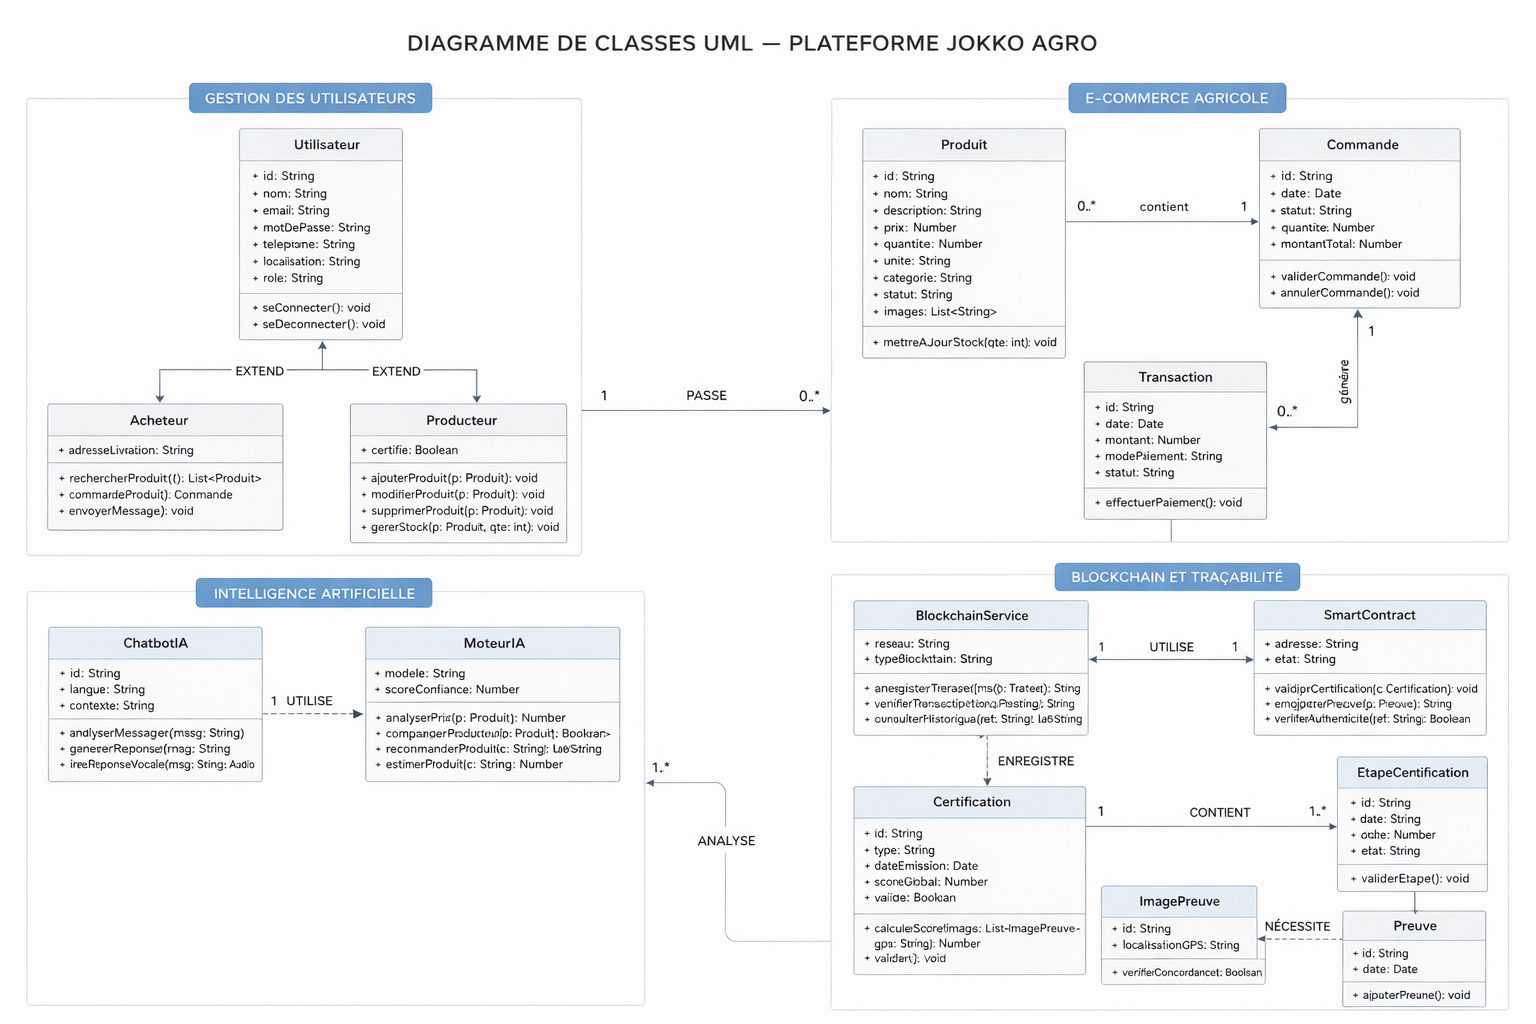
\includegraphics[width=1.0\textwidth,keepaspectratio]{images/diagramme_uml.png}
\caption{Diagramme de classes UML --- Architecture modulaire complète de Jokko Agro}
\label{fig:uml}
\end{figure}

\vspace{0.5cm}

\section{Diagrammes de séquence}

\subsection{Séquence Blockchain}

\noindent
Le diagramme suivant illustre le flux complet de certification d'un produit agricole,
depuis la prise de photo par l'agriculteur jusqu'à l'enregistrement on-chain.

\vspace{0.3cm}

\begin{figure}[H]
\centering
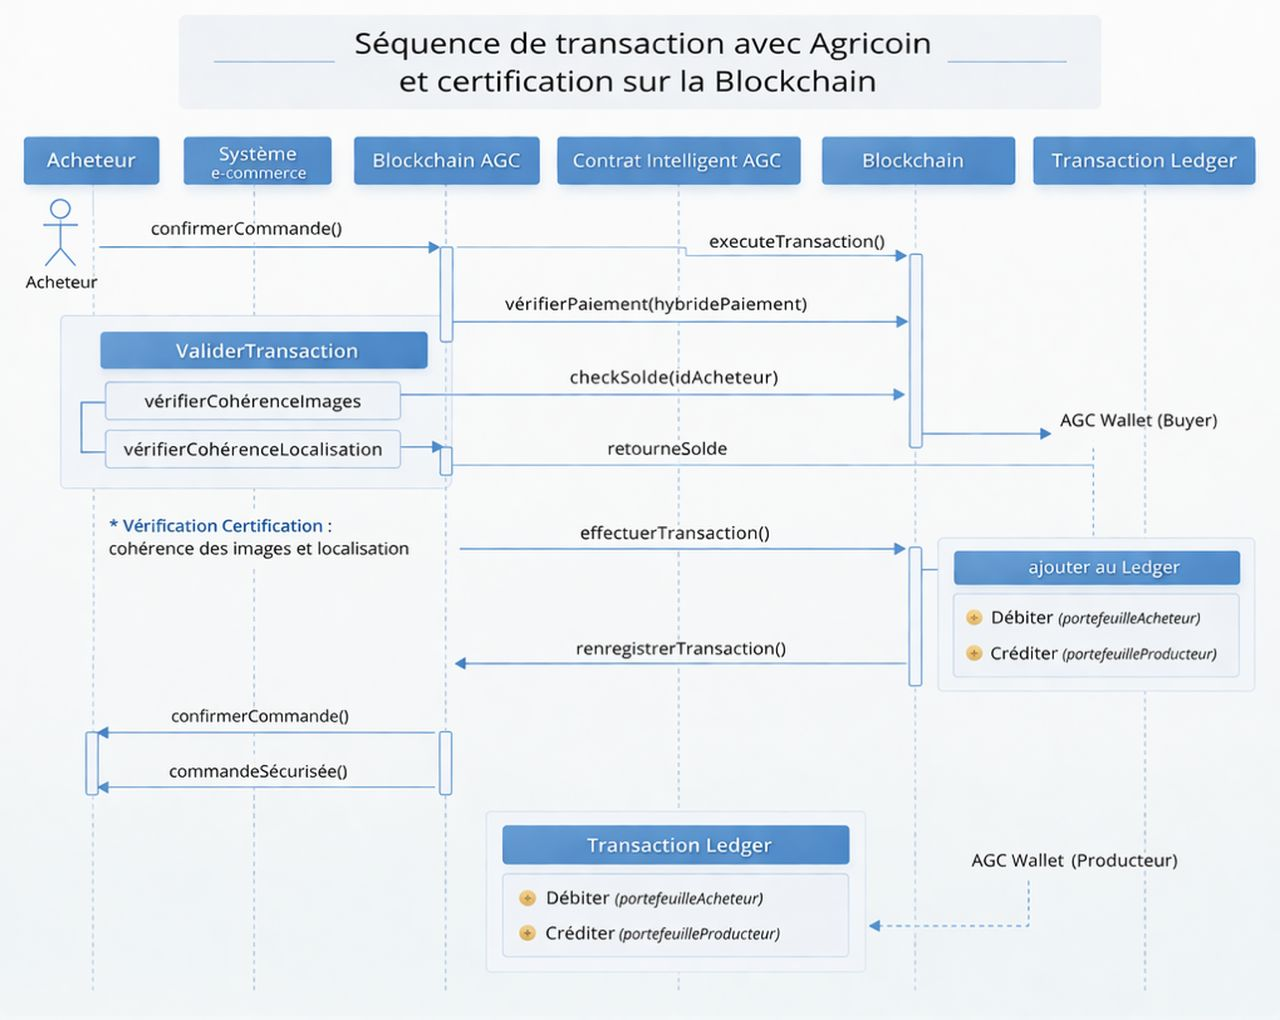
\includegraphics[width=1.0\textwidth,keepaspectratio]{images/diagramme_sequence_blockchain.jpeg}
\caption{Diagramme de séquence --- Flux de certification blockchain}
\label{fig:seq_bc}
\end{figure}

\vspace{0.3cm}

\noindent
Le flux se déroule en \textbf{six étapes} : (1) prise de photo + validation GPS, (2) calcul
du hash SHA-256, (3) upload IPFS via Pinata, (4) construction de l'objet canonique,
(5) envoi de la transaction Ethereum signée MetaMask, (6) enregistrement du résultat dans
Firestore.

\vspace{0.4cm}

\subsection{Séquence IA}

\noindent
Ce diagramme décrit l'interaction entre l'utilisateur et le chatbot, en montrant
le traitement de la voix Wolof, l'appel à l'API Claude et le retour de la réponse.

\vspace{0.3cm}

\begin{figure}[H]
\centering
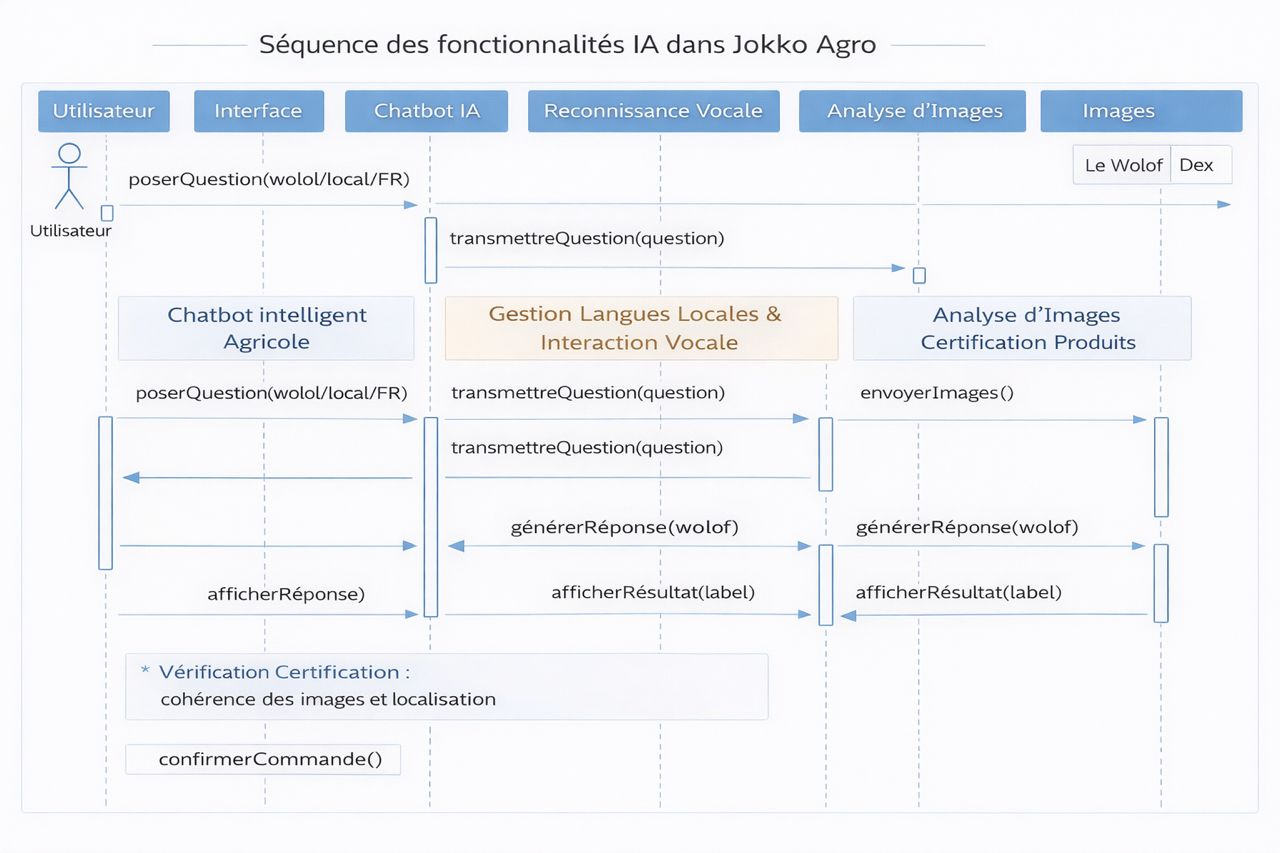
\includegraphics[width=1.0\textwidth,keepaspectratio]{images/diagramme_sequence_ia.jpeg}
\caption{Diagramme de séquence --- Interaction utilisateur avec l'IA}
\label{fig:seq_ia}
\end{figure}

\vspace{0.4cm}

\section{Flux de données}

\noindent
Les quatre axes de Jokko Agro échangent des données à des points clés. Ces interactions
sont essentielles à la cohérence du système :

\vspace{0.3cm}

\begin{tcolorbox}[infobox,title={Interactions inter-axes}]
\begin{itemize}[itemsep=6pt]
  \item \textbf{IA $\leftrightarrow$ Blockchain :} le service
        \texttt{image\_comparison\_service} valide la photo \textit{avant} que
        \texttt{blockchain\_service} l'enregistre sur IPFS. Les coordonnées GPS
        validées sont incluses dans le hash de preuve canonique.
  \item \textbf{Blockchain $\leftrightarrow$ Sécurité :} chaque enregistrement
        on-chain est précédé d'une signature ECDSA et journalisé dans l'Audit Trail.
        Le Ledger SHA-256 trace tous les états de certification.
  \item \textbf{AGC $\leftrightarrow$ Blockchain :} un bonus AGC est crédité
        automatiquement lors d'une certification réussie. Le cycle
        lock/release du séquestre est enregistré dans le Ledger.
  \item \textbf{Sécurité $\leftrightarrow$ Tous :} les transactions atomiques
        Firestore protègent AGC et Blockchain. L'Audit Trail couvre les quatre axes.
\end{itemize}
\end{tcolorbox}

\vspace{0.5cm}

\section{Scalabilité et déploiement}

\noindent
L'architecture de Jokko Agro est conçue pour évoluer. Plusieurs dimensions de
scalabilité sont prises en compte :

\vspace{0.3cm}

\begin{tcolorbox}[infobox,title={Perspectives de scalabilité}]
\begin{itemize}[itemsep=5pt]
  \item \textbf{Firebase Auto-scaling :} Firestore scale automatiquement en fonction
        du nombre de connexions, sans intervention manuelle.
  \item \textbf{Layer 2 Ethereum :} migration prévue vers \textbf{Polygon} pour
        réduire les frais de transaction (gas fees) lors du passage en production.
  \item \textbf{Multilangue :} l'architecture du chatbot permet d'ajouter d'autres
        langues (Pulaar, Sérère) sans refonte, en modifiant uniquement le prompt système.
  \item \textbf{Modèle de données extensible :} les collections Firestore sont conçues
        pour absorber de nouveaux types de certifications sans migration de schéma.
\end{itemize}
\end{tcolorbox}

% =========================================================
%  CHAPITRE 5 — INTELLIGENCE ARTIFICIELLE (RÉDUIT POUR LA LONGUEUR)
% =========================================================
\chapter{Axe Intelligence Artificielle}

\begin{tcolorbox}[chapterbox,title={Vue d'ensemble du chapitre}]
L'axe IA regroupe quatre services : le chatbot agricole bilingue, la reconnaissance
vocale en Wolof, la comparaison d'images anti-fraude, et la géolocalisation intelligente.
Ensemble, ils rendent Jokko Agro accessible aux agriculteurs quelle que soit leur maîtrise
du numérique.
\end{tcolorbox}

\vspace{0.5cm}

\section{Présentation de l'axe IA}

\noindent
L'axe IA de Jokko Agro comprend \textbf{quatre services Angular} spécialisés, tous
orientés vers l'assistance des agriculteurs.

\begin{figure}[H]
\centering
\begin{tikzpicture}[font=\small]

\draw[fill=bleuUniv, draw=bleuUniv] (0,0) circle (0.9cm);
\node[text=white, font=\bfseries\small] at (0,0) {Axe IA};

\draw[fill=bleuTresClair, draw=bleuUniv, rounded corners=5pt] (-5,2.5) rectangle (0,3.9);
\node[text width=4.6cm, align=center, font=\bfseries\small] at (-2.5,3.2) {chatbot\_service};
\node[text width=4.6cm, align=center] at (-2.5,-3.2) {Assistant agricole FR/Wolof};

\draw[fill=bleuTresClair, draw=bleuUniv, rounded corners=5pt] (0,2.5) rectangle (5,3.9);
\node[text width=4.6cm, align=center, font=\bfseries\small] at (2.5,3.2) {wolof\_voice\_service};
\node[text width=4.6cm, align=center] at (-2.5,-3.2) {Reconnaissance vocale Wolof};

\draw[fill=bleuPale, draw=bleuUniv, rounded corners=5pt] (-5,-3.9) rectangle (0,-2.5);
\node[text width=4.6cm, align=center, font=\bfseries\small] at (-2.5,-2.8) {image\_comparison\_service};
\node[text width=4.6cm, align=center] at (-2.5,-3.2) {Vision \& anti-fraude};

\draw[fill=bleuPale, draw=bleuUniv, rounded corners=5pt] (0,-3.9) rectangle (5,-2.5);
\node[text width=4.6cm, align=center, font=\bfseries\small] at (2.5,-2.8) {smart\_geolocation\_service};
\node[text width=4.6cm, align=center] at (2.5,-3.2) {GPS \& validation terrain};

\draw[->, bleuUniv, thick] (0,0.9) -- (-2.5,2.5);
\draw[->, bleuUniv, thick] (0,0.9) -- (2.5,2.5);
\draw[->, bleuUniv, thick] (0,-0.9) -- (-2.5,-2.5);
\draw[->, bleuUniv, thick] (0,-0.9) -- (2.5,-2.5);

\end{tikzpicture}
\caption{Les quatre services de l'axe IA}
\label{fig:axe_ia}
\end{figure}

\vspace{0.5cm}

\section{Chatbot agricole intelligent}

\noindent
Le chatbot est le point d'entrée principal de l'assistance agricole. Il permet des
conversations en \textbf{français et en Wolof} pour obtenir des conseils agronomiques
personnalisés, adaptés aux cultures et aux conditions climatiques du Sénégal.

\vspace{0.3cm}

\begin{tcolorbox}[infobox,title={Caractéristiques du chatbot}]
\begin{itemize}[itemsep=5pt]
  \item \textbf{Moteur LLM :} API Claude d'Anthropic (\texttt{claude-sonnet})
  \item \textbf{Prompt système :} orienté agronomie sénégalaise (cultures locales,
        saisons, parasites, irrigation)
  \item \textbf{Historique de conversation :} maintenu côté client (array de messages),
        transmis à chaque requête pour des échanges cohérents sur plusieurs tours
  \item \textbf{Bilingue natif :} le modèle gère nativement le Wolof et répond dans
        la langue de l'utilisateur
\end{itemize}
\end{tcolorbox}

\vspace{0.4cm}

\begin{figure}[H]
\centering
\begin{tikzpicture}[font=\small]

\draw[fill=bleuTresClair, draw=bleuUniv, rounded corners=4pt] (0,0) rectangle (3.5,1);
\node[align=center] at (1.75,0.5) {Utilisateur\\(FR ou Wolof)};

\draw[fill=bleuTresClair, draw=bleuUniv, rounded corners=4pt] (4,0) rectangle (7.5,1);
\node[align=center] at (5.75,0.5) {Historique\\conversation};

\draw[fill=bleuTresClair, draw=bleuUniv, rounded corners=4pt] (8,0) rectangle (11.5,1);
\node[align=center] at (9.75,0.5) {Claude API\\(Anthropic)};

\draw[fill=bleuTresClair, draw=bleuUniv, rounded corners=4pt] (12,0) rectangle (15.5,1);
\node[align=center] at (13.75,0.5) {Réponse enrichie\\affichée};

\draw[->, bleuUniv, thick] (3.5,0.5) -- (4,0.5) node[midway,above,font=\tiny]{message};
\draw[->, bleuUniv, thick] (7.5,0.5) -- (8,0.5) node[midway,above,font=\tiny]{messages[]};
\draw[->, bleuUniv, thick] (11.5,0.5) -- (12,0.5) node[midway,above,font=\tiny]{conseil};

\node[draw=bleuUniv!50, rounded corners, fill=white, font=\footnotesize\itshape, text width=8cm, align=center] at (7.75,-1.5)
    {Exemple : \textit{«~Ndax mango bi dafa am problème ci sunuy?~»}\\
    $\Rightarrow$ Conseil en Wolof sur les parasites de la mangue};

\end{tikzpicture}
\caption{Flux de traitement du chatbot agricole}
\label{fig:chatbot_flux}
\end{figure}

\vspace{0.5cm}

\section{Reconnaissance vocale (Wolof)}

\noindent
Le service de reconnaissance vocale permet aux agriculteurs analphabètes ou peu à l'aise
avec le texte de \textbf{dicter leurs questions}. Le service fonctionne en trois étapes :

\begin{enumerate}[leftmargin=*,itemsep=6pt]
  \item \textbf{Capture audio :} \texttt{getUserMedia} + \texttt{SpeechRecognition API}
        pour obtenir une transcription brute.
  \item \textbf{Post-traitement phonologique :} une couche de normalisation traite les
        phonèmes spécifiques au Wolof (sons aspirés, tons) absents du support standard
        de la Web Speech API.
  \item \textbf{Transmission :} le texte normalisé est envoyé au \texttt{chatbot\_service}
        comme s'il avait été saisi manuellement.
\end{enumerate}

\begin{tcolorbox}[definbox]
\textbf{\color{bleuUniv}Défi technique :} La Web Speech API de Google ne supporte pas
officiellement le Wolof. Jokko Agro implémente une couche de post-traitement propriétaire
qui corrige les erreurs les plus fréquentes dans la transcription automatique du Wolof à
partir des modèles français.
\end{tcolorbox}

\vspace{0.5cm}

\section{Analyse d'images}

\noindent
Le service \texttt{image\_comparison\_service} est au cœur de l'anti-fraude. Il vérifie
la \textbf{cohérence visuelle} entre les photos soumises à différentes étapes de
certification. Il utilise \textbf{TensorFlow.js} (exécuté côté navigateur, sans serveur)
et calcule cinq métriques :

\vspace{0.3cm}

\renewcommand{\arraystretch}{1.5}
\begin{tcolorbox}[tablebox]
\begin{tabularx}{\textwidth}{
  >{\bfseries\small\color{bleuUniv}}p{3.5cm}
  >{\small\bfseries}p{2.8cm}
  >{\small}X
  >{\small\bfseries}p{1.2cm}}
\rowcolor{bleuUniv}
\multicolumn{1}{>{\bfseries\color{white}\small}p{3.5cm}}{Métrique} &
\multicolumn{1}{>{\bfseries\color{white}\small}p{2.8cm}}{Méthode} &
\multicolumn{1}{>{\bfseries\color{white}\small}X}{Usage} &
\multicolumn{1}{>{\bfseries\color{white}\small}p{1.2cm}}{Poids} \\
Similarité struct. & MSE               & Détecter les photos copiées & 0.30 \\
\rowcolor{bleuTresClair}
Similarité features & Cosinus (embed.) & Identifier le même produit  & 0.40 \\
Cohérence couleurs  & Histogramme HSV  & Vérifier maturité / saison  & 0.20 \\
\rowcolor{bleuTresClair}
Cohérence éclairage & Variance pixel   & Anti-spoofing               & 0.10 \\
\end{tabularx}
\end{tcolorbox}

\vspace{0.3cm}

\noindent
Le score final est calculé comme :
$$ \text{score} = 0.3 \times \text{MSE} + 0.4 \times \cos + 0.2 \times \text{HSV} + 0.1 \times \text{var} $$

\noindent
Selon le score : \textbf{accept} (conforme), \textbf{review} (vérification manuelle),
ou \textbf{reject} (fraude probable).

\vspace{0.5cm}

\section{Géolocalisation intelligente}

\noindent
Le service \texttt{smart\_geolocation\_service} valide que les photos de certification
sont bien prises \textbf{sur le terrain déclaré}, empêchant les certifications à distance.

\begin{tcolorbox}[infobox,title={Mécanismes de validation GPS}]
\begin{enumerate}[leftmargin=*,label=\textcolor{bleuUniv}{\textbf{V\arabic*.}},itemsep=5pt]
  \item \textbf{Cohérence de position :} distance entre coordonnées GPS actuelles
        et coordonnées du checkpoint enregistré $\leq$ rayon de tolérance (500 m).
  \item \textbf{Précision GPS :} \texttt{accuracy} $\leq$ seuil maximal accepté
        (ex: 100 m) pour rejeter les signaux de mauvaise qualité.
  \item \textbf{Anti-spoofing temporel :} cohérence entre l'horodatage GPS
        (\texttt{position.timestamp}) et l'heure réelle du système pour détecter
        les coordonnées figées ou rejouées.
\end{enumerate}
\end{tcolorbox}

\vspace{0.5cm}

\section{Apports de l'IA dans le système}

\begin{tcolorbox}[synthbox]
\textbf{Synthèse de l'axe IA}\\[6pt]
L'axe IA transforme Jokko Agro en une plateforme réellement accessible : le chatbot
supprime la barrière de l'expertise agronomique, la voix élimine la barrière de
l'alphabétisation, l'analyse d'images renforce l'intégrité de la certification, et
la géolocalisation garantit l'authenticité terrain. Ensemble, ces quatre services
rendent la plateforme utilisable par n'importe quel agriculteur sénégalais.
\end{tcolorbox}

% =========================================================
%  CHAPITRE 6 — BLOCKCHAIN ET CERTIFICATION (RÉDUIT)
% =========================================================
\chapter{Axe Blockchain et Certification}

\begin{tcolorbox}[chapterbox,title={Vue d'ensemble du chapitre}]
L'axe Blockchain est le pilier de confiance de Jokko Agro. Il permet d'enregistrer de
façon immuable et décentralisée les preuves de certification des produits agricoles, du
semis à la récolte, via Ethereum, IPFS et un smart contract Solidity.
\end{tcolorbox}

\vspace{0.5cm}

\section{Concept de blockchain}

\noindent
Une \textbf{blockchain} est une base de données distribuée dans laquelle les enregistrements
(blocs) sont liés cryptographiquement les uns aux autres, formant une chaîne immuable. Toute
modification d'un bloc passé invalide tous les blocs suivants, rendant la fraude détectable
immédiatement.

\vspace{0.4cm}

\begin{figure}[H]
\centering
\begin{tikzpicture}[font=\small,
  bloc/.style={rectangle,rounded corners=4pt,minimum width=3.2cm,minimum height=2.4cm,
               text centered,text width=3cm,draw=bleuUniv,line width=1pt,fill=bleuTresClair}]

  \node[bloc] (B0) at (0,0) {
    \textbf{\small Bloc \#0}\\[4pt]
    \footnotesize Hash: \texttt{000...}\\
    Prev: \texttt{---}\\
    Data: genesis
  };
  \node[bloc] (B1) at (4.2,0) {
    \textbf{\small Bloc \#1}\\[4pt]
    \footnotesize Hash: \texttt{a3f...}\\
    Prev: \texttt{000...}\\
    Data: cert\#1
  };
  \node[bloc] (B2) at (8.4,0) {
    \textbf{\small Bloc \#2}\\[4pt]
    \footnotesize Hash: \texttt{7bc...}\\
    Prev: \texttt{a3f...}\\
    Data: cert\#2
  };
  \node[bloc,draw=bleuUniv!50,fill=white] (B3) at (12.6,0) {
    \textbf{\small Bloc \#n}\\[4pt]
    \footnotesize Hash: \texttt{...}\\
    Prev: \texttt{7bc...}\\
    Data: cert\#n
  };

  \draw[-{Stealth},bleuUniv,thick] (B0.east)--(B1.west);
  \draw[-{Stealth},bleuUniv,thick] (B1.east)--(B2.west);
  \draw[-{Stealth},bleuUniv!50,thick,dashed] (B2.east)--(B3.west);

  \draw[bleuUniv!60,decorate,decoration={brace,amplitude=6pt,mirror}]
    (0,-1.5)--(12.6,-1.5) node[midway,below=8pt,font=\small\itshape,bleuUniv]
    {Chaîne immuable --- toute modification est détectée};
\end{tikzpicture}
\caption{Structure d'une blockchain --- principe de chaînage par hash}
\label{fig:blockchain}
\end{figure}

\vspace{0.5cm}

\section{Smart Contract de certification}

\noindent
Le contrat \texttt{CertificationRegistry.sol} est le cœur de la traçabilité. Déployé sur
le réseau Ethereum Sepolia, il stocke de façon permanente les preuves de certification avec
les garanties suivantes :

\vspace{0.3cm}

\begin{tcolorbox}[infobox,title={Garanties du Smart Contract}]
\begin{itemize}[itemsep=5pt]
  \item \textbf{Immuabilité :} une preuve enregistrée ne peut jamais être modifiée
        ou supprimée.
  \item \textbf{Non-répudiation :} \texttt{msg.sender} (adresse Ethereum de l'appelant)
        est automatiquement stocké, liant chaque certification à son auteur de façon
        cryptographiquement prouvable.
  \item \textbf{Horodatage blockchain :} \texttt{block.timestamp} est fourni par le
        réseau, non par l'utilisateur --- il ne peut pas être falsifié.
  \item \textbf{Indexation :} l'événement \texttt{ProofRegistered} est indexé sur
        \texttt{productId}, permettant des recherches rapides sans parcourir toute la
        chaîne.
\end{itemize}
\end{tcolorbox}

\vspace{0.5cm}

\section{Enregistrement des preuves}

\noindent
Le flux complet de certification coordonne trois services Angular :

\vspace{0.4cm}

\begin{figure}[H]
\centering
\begin{tikzpicture}[font=\small]

\draw[fill=bleuUniv, draw=bleuUniv, rounded corners=4pt, text=white] (0,6.5) rectangle (4,7.4);
\node[align=center, text=white] at (2,6.95) {1. Photo uploadée};

\draw[fill=bleuTresClair, draw=bleuUniv, rounded corners=4pt] (0,5.3) rectangle (4,6.2);
\node[align=center] at (2,5.75) {2. Hash SHA-256 calculé};

\draw[fill=bleuTresClair, draw=bleuUniv, rounded corners=4pt] (0,4.1) rectangle (4,5);
\node[align=center] at (2,4.55) {3. Upload IPFS $\rightarrow$ CID};

\draw[fill=bleuTresClair, draw=bleuUniv, rounded corners=4pt] (0,2.9) rectangle (4,3.8);
\node[align=center] at (2,3.35) {4. Objet canonique créé};

\draw[fill=bleuTresClair, draw=bleuUniv, rounded corners=4pt] (0,1.7) rectangle (4,2.6);
\node[align=center] at (2,2.15) {5. Hash final (proofHash)};

\draw[fill=bleuMoyen, draw=bleuUniv, rounded corners=4pt, text=white] (0,0.5) rectangle (4,1.4);
\node[align=center, text=white] at (2,0.95) {6. Transaction Sepolia};

\draw[fill=bleuPale, draw=bleuUniv, rounded corners=4pt] (0,-0.7) rectangle (4,0.2);
\node[align=center] at (2,-0.25) {7. Résultat $\rightarrow$ Firestore};

\draw[->, bleuUniv, thick] (2,6.5) -- (2,6.2);
\draw[->, bleuUniv, thick] (2,5.3) -- (2,5);
\draw[->, bleuUniv, thick] (2,4.1) -- (2,3.8);
\draw[->, bleuUniv, thick] (2,2.9) -- (2,2.6);
\draw[->, bleuUniv, thick] (2,1.7) -- (2,1.4);
\draw[->, bleuUniv, thick] (2,0.5) -- (2,0.2);

\node[font=\tiny\itshape, bleuUniv, anchor=west] at (4.2,5.75) {\texttt{CryptoJS.SHA256(photoBuffer)}};
\node[font=\tiny\itshape, bleuUniv, anchor=west] at (4.2,4.55) {\texttt{ipfs\_service.uploadFile()} $\rightarrow$ CIDv1};
\node[font=\tiny\itshape, bleuUniv, anchor=west] at (4.2,3.35) {\texttt{\{productId, hash, lat, lng, step\}}};
\node[font=\tiny\itshape, bleuUniv, anchor=west] at (4.2,2.15) {\texttt{SHA256(JSON.stringify(canonical))}};
\node[font=\tiny\itshape, bleuUniv, anchor=west] at (4.2,0.95) {\texttt{registerProof()} $\rightarrow$ txHash};

\end{tikzpicture}
\caption{Flux complet de création d'une preuve de certification}
\label{fig:flux_cert}
\end{figure}

\vspace{0.5cm}

\section{Interaction avec Ethereum}

\noindent
Le service \texttt{ethereum\_service} gère toutes les interactions avec MetaMask et le
réseau Ethereum via Alchemy RPC :

\vspace{0.3cm}

\begin{tcolorbox}[infobox,title={Méthodes clés de l'ethereum\_service}]
\begin{itemize}[itemsep=4pt,font=\small]
  \item \texttt{connectWallet()} --- \texttt{eth\_requestAccounts} $\rightarrow$ popup MetaMask
  \item \texttt{checkNetwork(11155111)} --- vérifie que l'utilisateur est sur Sepolia
  \item \texttt{switchNetwork(11155111)} --- bascule automatiquement sur Sepolia
  \item \texttt{encodeContractCall(ABI, 'registerProof', params)} --- encodage ABI
  \item \texttt{sendContractTransaction(addr, data)} --- envoi transaction signée
  \item \texttt{getTransactionReceipt(txHash)} --- suivi confirmation (status 0x1)
\end{itemize}
\end{tcolorbox}

\vspace{0.5cm}

\section{Stockage IPFS}

\noindent
Les photos de certification sont stockées sur \textbf{IPFS via Pinata}, garantissant
leur accessibilité décentralisée. Le CIDv1 produit des identifiants stables, résistants
aux collisions.

\vspace{0.3cm}

\begin{tcolorbox}[infobox,title={Méthodes de l'ipfs\_service}]
\begin{itemize}[itemsep=4pt]
  \item \texttt{uploadFile(file)} $\rightarrow$ \texttt{\{cid, url\}} --- photo vers IPFS
  \item \texttt{uploadJSON(data)} $\rightarrow$ \texttt{\{cid, url\}} --- métadonnées vers IPFS
  \item \texttt{verifyCID(cid)} $\rightarrow$ \texttt{boolean} --- vérification existence
  \item \texttt{getGatewayUrl(cid)} $\rightarrow$ \texttt{string} --- URL CDN Pinata
\end{itemize}
\end{tcolorbox}

\vspace{0.5cm}

\section{Traçabilité et transparence}

\noindent
La certification s'organise en \textbf{7 checkpoints} couvrant le cycle complet de
production agricole, avec un système de badges récompensant la qualité :

\begin{figure}[H]
\centering
\begin{tikzpicture}[font=\small]

% Checkpoints ligne 1
\draw[fill=bleuTresClair, draw=bleuUniv, rounded corners=3pt] (0,0) rectangle (2.4,0.9);
\node[align=center, font=\footnotesize\bfseries] at (1.2,0.45) {Préparation du sol};

\draw[fill=bleuTresClair, draw=bleuUniv, rounded corners=3pt] (2.8,0) rectangle (5.2,0.9);
\node[align=center, font=\footnotesize\bfseries] at (4,0.45) {Semis};

\draw[fill=bleuTresClair, draw=bleuUniv, rounded corners=3pt] (5.6,0) rectangle (8,0.9);
\node[align=center, font=\footnotesize\bfseries] at (6.8,0.45) {Irrigation};

\draw[fill=bleuTresClair, draw=bleuUniv, rounded corners=3pt] (8.4,0) rectangle (10.8,0.9);
\node[align=center, font=\footnotesize\bfseries] at (9.6,0.45) {Traitements};

\draw[fill=bleuTresClair, draw=bleuUniv, rounded corners=3pt] (11.2,0) rectangle (13.6,0.9);
\node[align=center, font=\footnotesize\bfseries] at (12.4,0.45) {Surveillance};

% Checkpoints ligne 2
\draw[fill=bleuTresClair, draw=bleuUniv, rounded corners=3pt] (9.8,-2) rectangle (12.2,-1.1);
\node[align=center, font=\footnotesize\bfseries] at (11,-1.55) {Récolte};

\draw[fill=bleuTresClair, draw=bleuUniv, rounded corners=3pt] (7,-2) rectangle (9.4,-1.1);
\node[align=center, font=\footnotesize\bfseries] at (8.2,-1.55) {Stockage};

% Flèches horizontales
\draw[->, bleuUniv, thick] (2.4,0.45) -- (2.8,0.45);
\draw[->, bleuUniv, thick] (5.2,0.45) -- (5.6,0.45);
\draw[->, bleuUniv, thick] (8,0.45) -- (8.4,0.45);
\draw[->, bleuUniv, thick] (10.8,0.45) -- (11.2,0.45);

% Flèches verticales
\draw[->, bleuUniv, thick] (12.4,0) -- (12.4,-0.8) -- (11,-1.1);
\draw[->, bleuUniv, thick] (11,-1.1) -- (9.8,-1.55) -- (8.2,-1.55);

% Badges
\draw[bleuUniv, dashed, rounded corners] (-0.2,-3.2) rectangle (3.5,-2.6);
\node[font=\footnotesize\bfseries, bleuUniv] at (1.65,-2.9) {Bronze (0--40 pts)};

\draw[bleuUniv, dashed, rounded corners] (3.8,-3.2) rectangle (7.6,-2.6);
\node[font=\footnotesize\bfseries, bleuUniv] at (5.7,-2.9) {Silver (41--70 pts)};

\draw[fill=bleuUniv, draw=bleuUniv, rounded corners] (7.9,-3.2) rectangle (12.6,-2.6);
\node[font=\footnotesize\bfseries, white] at (10.25,-2.9) {Gold (71--100 pts)};

\end{tikzpicture}
\caption{Les 7 checkpoints de certification et le système de badges}
\label{fig:checkpoints}
\end{figure}

% =========================================================
%  CHAPITRE 7 — AGRICOINS (AGC) ET DATAWAREHOUSE
% =========================================================
\chapter{Système Agricoins (AGC) et Datawarehouse}

\begin{tcolorbox}[chapterbox,title={Vue d'ensemble du chapitre}]
L'axe Agricoins crée un écosystème économique incitatif au sein de Jokko Agro. Il combine
une monnaie numérique agricole (AGC), un système de paiement hybride sécurisé, un module
commerce complet et un datawarehouse d'aide à la décision.
\end{tcolorbox}

\vspace{0.5cm}

\section{Présentation des Agricoins}

\noindent
L'\textbf{Agricoin (AGC)} est la monnaie numérique interne de Jokko Agro. Sa création
répond à trois objectifs : simplifier les micro-transactions agricoles, inciter les
bonnes pratiques via des récompenses, et créer un lien direct entre certification et
valeur économique.

\vspace{0.3cm}

\begin{tcolorbox}[infobox,title={Parité et sources d'AGC}]
\begin{center}
\large\bfseries\color{bleuUniv} 1 AGC = 100 FCFA (parité fixe)
\end{center}
\vspace{0.3cm}
\begin{itemize}[itemsep=5pt]
  \item \textbf{Achat direct :} via Wave, Orange Money ou Free
  \item \textbf{Récompense de certification :} bonus AGC crédité automatiquement
        à chaque checkpoint blockchain validé
  \item \textbf{Solde initial :} émission à l'inscription pour les nouveaux utilisateurs
\end{itemize}
\end{tcolorbox}

\vspace{0.5cm}

\begin{figure}[H]
\centering
\begin{minipage}{0.48\textwidth}
\centering
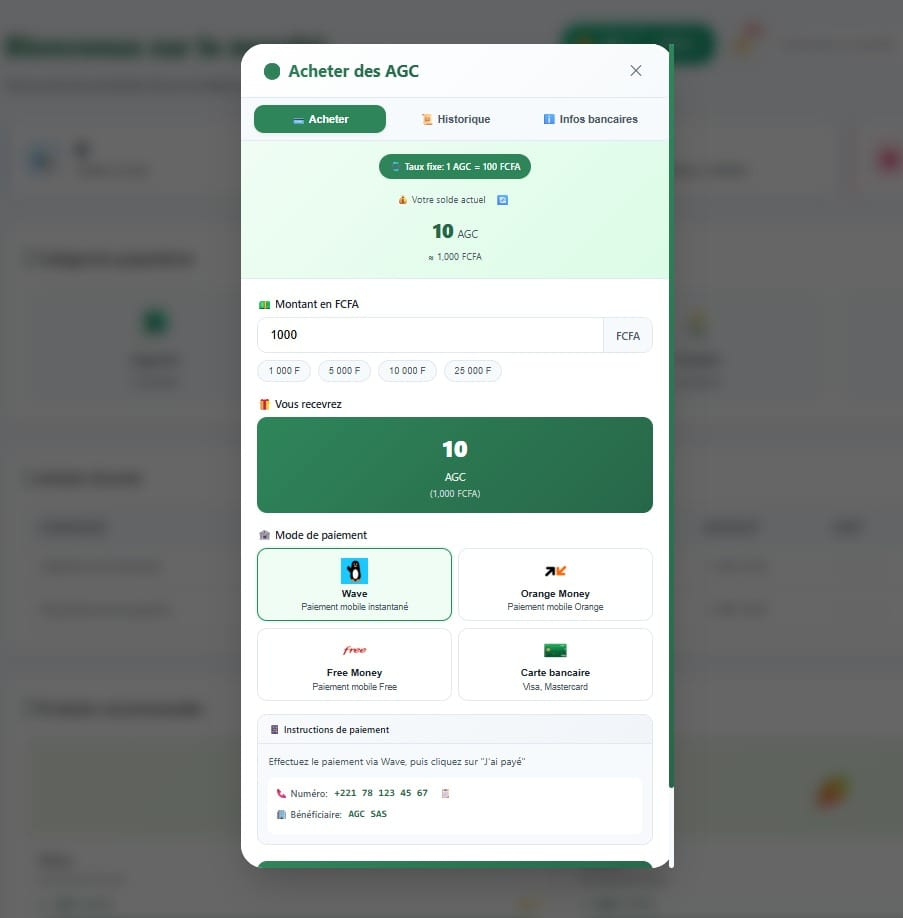
\includegraphics[width=\textwidth]{images/agc1.jpeg}
\caption{Interface d'achat des Agricoins (AGC)}
\label{fig:agc_achat}
\end{minipage}
\hfill
\begin{minipage}{0.48\textwidth}
\centering
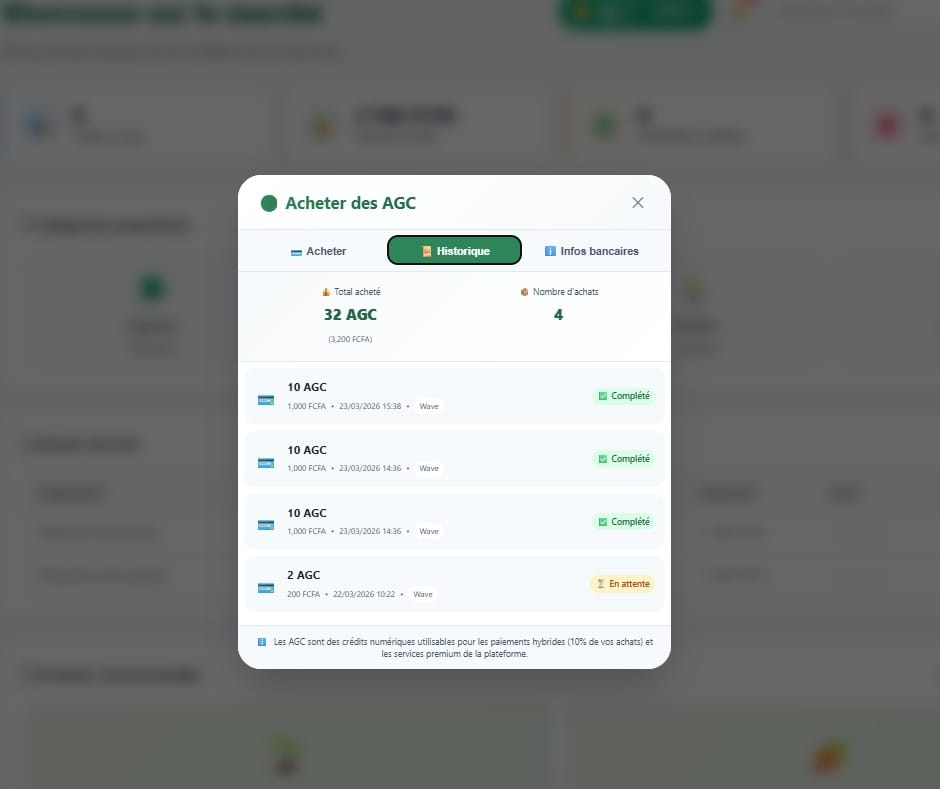
\includegraphics[width=\textwidth]{images/agc2.jpeg}
\caption{Historique des transactions AGC}
\label{fig:agc_historique}
\end{minipage}
\end{figure}

\vspace{0.3cm}

\noindent
L'interface d'achat permet aux utilisateurs d'acquérir des AGC via les plateformes de
mobile money (Wave, Orange Money, Free) ou par carte bancaire. Le taux de conversion
est fixe : \textbf{1 AGC = 100 FCFA}. L'historique des transactions permet de suivre
l'ensemble des achats effectués, avec le statut de chaque transaction (Complété / En attente).

\vspace{0.5cm}

\section{Mécanisme d'émission}

\noindent
Le solde AGC de chaque utilisateur est stocké dans Firestore sous la structure suivante :

\vspace{0.3cm}

\begin{tcolorbox}[infobox,title={Structure Firestore du portefeuille AGC}]
\begin{lstlisting}[basicstyle=\footnotesize\ttfamily]
users/{uid}/
  agc_balance: number          // Solde courant en AGC
  agc_transactions[]:
    type: 'credit' | 'debit'
    amount: number             // Montant en AGC
    fiatAmount: number         // Equivalent FCFA
    timestamp: Timestamp
    reason: string             // 'CERTIFICATION_REWARD' | 'PURCHASE' | ...
    txHash?: string            // Hash ledger si applicable
\end{lstlisting}
\end{tcolorbox}

\vspace{0.5cm}

\section{Paiement hybride (AGC + Mobile Money)}

\noindent
Le système de paiement hybride permet de combiner AGC et mobile money pour régler une
commande. Un mécanisme de \textbf{séquestre (escrow)} protège acheteur et vendeur.

\vspace{0.4cm}

\begin{figure}[H]
\centering
\begin{tikzpicture}[font=\small,
  etape/.style={rectangle,rounded corners=4pt,minimum width=4.5cm,minimum height=1cm,
                text centered,text width=4.2cm,draw=bleuUniv,line width=0.8pt},
  arr/.style={-{Stealth},bleuUniv,thick}]

  \node[etape,fill=bleuUniv,text=white] (E1) at (0,5.5)
    {1. Acheteur passe commande};
  \node[etape,fill=bleuMoyen,text=white] (E2) at (0,4.2)
    {2. Lock AGC (séquestre)};
  \node[etape,fill=bleuTresClair] (E3) at (0,2.9)
    {3. Livraison en cours};
  \node[etape,fill=bleuTresClair] (E4a) at (-3,1.6)
    {4a. Livraison confirmée};
  \node[etape,fill=bleuTresClair] (E4b) at (3,1.6)
    {4b. Litige déclaré};
  \node[etape,fill=bleuPale] (E5a) at (-3,0.3)
    {Release AGC $\rightarrow$ Producteur};
  \node[etape,fill=bleuPale] (E5b) at (3,0.3)
    {Rollback $\rightarrow$ Acheteur};
  \node[etape,fill=bleuUniv!20] (E6) at (0,-1.0)
    {5. DW mis à jour};

  \draw[arr] (E1.south)--(E2.north);
  \draw[arr] (E2.south)--(E3.north);
  \draw[arr] (E3.south west)--(E4a.north);
  \draw[arr] (E3.south east)--(E4b.north);
  \draw[arr] (E4a.south)--(E5a.north);
  \draw[arr] (E4b.south)--(E5b.north);
  \draw[arr] (E5a.south east)--(E6.north west);
  \draw[arr] (E5b.south west)--(E6.north east);

  % Escrow box
  \draw[bleuMoyen,dashed,rounded corners] (-2.7,1.3) rectangle (2.7,4.6);
  \node[font=\tiny\itshape,bleuMoyen] at (0,4.45) {Zone Séquestre};
\end{tikzpicture}
\caption{Cycle de vie d'un paiement AGC avec escrow}
\label{fig:escrow}
\end{figure}

\vspace{0.5cm}

\section{Gestion des transactions}

\noindent
Toutes les transactions AGC utilisent les \textbf{transactions atomiques Firestore}
(\texttt{runTransaction}), garantissant que le débit de l'acheteur et le crédit du
producteur s'effectuent toujours ensemble --- ou pas du tout en cas d'erreur réseau.

\vspace{0.3cm}

\begin{tcolorbox}[definbox]
\textbf{\color{bleuUniv}Propriétés ACID garanties :}
\textbf{Atomicité} (débit + crédit simultanés),
\textbf{Cohérence} (double dépense impossible, balance vérifiée atomiquement),
\textbf{Rollback automatique} (état précédent restauré en cas d'erreur).
\end{tcolorbox}

\vspace{0.5cm}

\section{Commerce et marketplace}

\noindent
Le module commerce gère le cycle complet d'une vente avec \textbf{7 états de commande} :

\vspace{0.3cm}

\begin{figure}[H]
\centering
\begin{tikzpicture}[font=\footnotesize,
  s/.style={rectangle,rounded corners=3pt,minimum width=2cm,minimum height=0.7cm,
            text centered,draw=bleuUniv,fill=bleuTresClair,line width=0.7pt},
  a/.style={-{Stealth},bleuUniv,thick}]

  \node[s] (s1) at (0,0)    {pending};
  \node[s] (s2) at (2.6,0)  {confirmed};
  \node[s] (s3) at (5.2,0)  {preparing};
  \node[s] (s4) at (7.8,0)  {ready};
  \node[s] (s5) at (10.4,1) {pickup};
  \node[s] (s6) at (10.4,-1){delivery};
  \node[s,fill=bleuMoyen,text=white] (s7) at (13,0) {completed};
  \node[s,fill=bleuPale] (s8) at (7.8,-2) {disputed};
  \node[s,fill=bleuPale] (s9) at (5.2,-2) {cancelled};

  \draw[a] (s1)--(s2); \draw[a] (s2)--(s3);
  \draw[a] (s3)--(s4);
  \draw[a] (s4.north east)--(s5.west);
  \draw[a] (s4.south east)--(s6.west);
  \draw[a] (s5.east)--(s7.north west);
  \draw[a] (s6.east)--(s7.south west);
  \draw[a] (s6.south)--(s8.east);
  \draw[a] (s8.west)--(s9.east);
\end{tikzpicture}
\caption{Machine à états d'une commande Jokko Agro}
\label{fig:etats_commande}
\end{figure}

\vspace{0.5cm}

\section{Datawarehouse agricole}

\noindent
Le datawarehouse agrège les données de ventes, paiements AGC et certifications pour
produire des \textbf{indicateurs de performance actionnables} pour les agriculteurs.

\vspace{0.3cm}

\renewcommand{\arraystretch}{1.5}
\begin{tcolorbox}[tablebox]
\begin{tabularx}{\textwidth}{
  >{\bfseries\small\color{bleuUniv}}p{2.8cm}
  >{\small}p{3.5cm}
  >{\small\ttfamily}X}
\rowcolor{bleuUniv}
\multicolumn{1}{>{\bfseries\color{white}\small}p{2.8cm}}{Catégorie} &
\multicolumn{1}{>{\bfseries\color{white}\small}p{3.5cm}}{Indicateur} &
\multicolumn{1}{>{\bfseries\color{white}\small}X}{Stockage Firestore} \\
Revenus        & Mensuel / Annuel          & \texttt{monthlyRevenue[]} \\
\rowcolor{bleuTresClair}
Performance    & Top produits / Top acheteurs & \texttt{dailyStats[]} \\
Qualité        & Taux complétion, note moy. & \texttt{weeklyTrend} \\
\rowcolor{bleuTresClair}
AGC            & Locked / Released          & Firestore real-time \\
Prévision      & Tendance revenus (trend)   & \texttt{predictedRevenue} \\
\rowcolor{bleuTresClair}
Temporel       & Pic d'heure / Meilleur jour & Agrégat Firestore \\
\end{tabularx}
\end{tcolorbox}

\vspace{0.5cm}

\section{Analyse et prévisions}

\noindent
Le module de prévision utilise une \textbf{moyenne mobile pondérée} sur les 12 derniers
mois de revenus pour produire une estimation des revenus futurs. Cette prévision est
stockée dans \texttt{predictedRevenue} et mise à jour à chaque nouvelle transaction.

\vspace{0.3cm}

\begin{figure}[H]
\centering
\begin{tikzpicture}[font=\small]
  % Axes
  \draw[bleuUniv,thick,->] (0,0)--(9.5,0) node[right]{Mois};
  \draw[bleuUniv,thick,->] (0,0)--(0,5) node[above,font=\tiny]{Revenus (FCFA)};

  % Données fictives réalistes
  \foreach \x/\y in {0.5/1.2,1.5/1.8,2.5/1.5,3.5/2.3,4.5/2.8,
                     5.5/2.4,6.5/3.1,7.5/3.5,8.5/3.8} {
    \fill[bleuUniv] (\x,\y) circle (2.5pt);
  }
  % Courbe réelle
  \draw[bleuUniv,thick]
    (0.5,1.2)--(1.5,1.8)--(2.5,1.5)--(3.5,2.3)--(4.5,2.8)
    --(5.5,2.4)--(6.5,3.1)--(7.5,3.5)--(8.5,3.8);

  % Prévision
  \draw[bleuClair,thick,dashed] (8.5,3.8)--(9.5,4.2);
  \fill[bleuClair] (9.5,4.2) circle (3pt);
  \node[font=\tiny\itshape,bleuClair,right] at (9.5,4.2) {prévision};

  % Légende
  \draw[bleuUniv,thick] (0.8,4.5)--(1.5,4.5);
  \node[font=\tiny,bleuUniv,right] at (1.5,4.5) {Revenus réels};
  \draw[bleuClair,thick,dashed] (0.8,4.1)--(1.5,4.1);
  \node[font=\tiny,bleuClair,right] at (1.5,4.1) {Prévision (moy. mobile)};

  % Mois labels
  \foreach \x/\m in {0.5/Jan,1.5/Fév,2.5/Mar,3.5/Avr,4.5/Mai,
                     5.5/Jun,6.5/Jul,7.5/Aoû,8.5/Sep}
    \node[font=\tiny,bleuUniv,below] at (\x,-0.1) {\m};
\end{tikzpicture}
\caption{Évolution et prévision des revenus dans le datawarehouse Jokko Agro}
\label{fig:prevision}
\end{figure}

% =========================================================
%  CHAPITRE 8 — SÉCURITÉ ET CRYPTOGRAPHIE (RÉDUIT)
% =========================================================
\chapter{Sécurité et Cryptographie}

\begin{tcolorbox}[chapterbox,title={Vue d'ensemble du chapitre}]
L'axe Sécurité est transversal à toute la plateforme. Il garantit l'intégrité des données,
l'authentification des acteurs et la confidentialité des informations sensibles à travers
dix mécanismes cryptographiques complémentaires, organisés en couches de défense.
\end{tcolorbox}

\vspace{0.5cm}

\section{Architecture de sécurité}

\noindent
La sécurité de Jokko Agro repose sur une architecture en \textbf{dix couches
complémentaires}, chacune adressant une menace spécifique. Cette approche de défense
en profondeur garantit que la compromission d'une couche n'entraîne pas celle de
l'ensemble du système.

\vspace{0.4cm}

\begin{figure}[H]
\centering
\begin{tikzpicture}[font=\small,
  couche/.style={rectangle,rounded corners=4pt,minimum width=12cm,minimum height=0.9cm,
                 text centered,draw=bleuUniv,line width=0.8pt,font=\footnotesize}]

  \node[couche,fill=bleuUniv,text=white]     at (0,7.2)
    {Couche 10 --- Tests d'intrusion --- Validation robustesse face aux attaques};
  \node[couche,fill=bleuUniv!90,text=white]  at (0,6.3)
    {Couche 9 --- Journalisation et Audit Trail --- Traçabilité complète};
  \node[couche,fill=bleuUniv!80,text=white]  at (0,5.4)
    {Couche 8 --- Chiffrement des données sensibles --- AES-GCM / HTTPS};
  \node[couche,fill=bleuUniv!70,text=white]  at (0,4.5)
    {Couche 7 --- Authentification forte (2FA) --- Double vérification};
  \node[couche,fill=bleuUniv!60,text=white]  at (0,3.6)
    {Couche 6 --- Détection d'anomalies comportementales --- ML temps réel};
  \node[couche,fill=bleuUniv!50,text=white]  at (0,2.7)
    {Couche 5 --- Rate limiting adaptatif --- Limitation dynamique};
  \node[couche,fill=bleuMoyen,text=white]    at (0,1.8)
    {Couche 4 --- Atomicité transactionnelle --- Rollback automatique};
  \node[couche,fill=bleuClair,text=white]    at (0,0.9)
    {Couche 3 --- Système de séquestre (Escrow) --- Protection AGC};
  \node[couche,fill=bleuUniv!40,text=white]  at (0,0)
    {Couche 2 --- Signatures numériques (ECDSA P-256) --- Non-répudiation};
  \node[couche,fill=bleuUniv!30,text=white]  at (0,-0.9)
    {Couche 1 --- Ledger immuable SHA-256 --- Intégrité historique};
\end{tikzpicture}
\caption{Architecture de sécurité en dix couches de Jokko Agro}
\label{fig:securite}
\end{figure}

\vspace{0.5cm}

\section{Ledger immuable (Couche 1)}

\noindent
Un \textbf{ledger local} (inspiré de la blockchain) chaîne chaque action sensible via
SHA-256, rendant toute modification rétroactive immédiatement détectable. Cette structure
de données chaînée garantit l'intégrité historique des transactions AGC.

\vspace{0.3cm}

\begin{tcolorbox}[infobox,title={Structure d'un bloc du ledger}]
\begin{lstlisting}[basicstyle=\footnotesize\ttfamily]
interface Block {
  previousHash: string;  // Hash du bloc precedent
  blockHeight:  number;  // Index sequentiel
  nonce:        number;  // Nonce anti-collision
  timestamp:    number;  // Horodatage UTC
  data:         any;     // Donnees de l'action
  hash:         string;  // SHA256(data+prev+ts+nonce)
}

// Regle d'integrite :
// Si block[n].hash != SHA256(block[n].data
//   + block[n-1].hash + timestamp + nonce)
// => TOUTE la chaine est invalidee
\end{lstlisting}
\end{tcolorbox}

\vspace{0.3cm}

\noindent
\textbf{Implémentation Firebase :} Le ledger est stocké dans la collection \texttt{ledger\_blocks}
avec des règles Firestore empêchant toute modification ultérieure.

\begin{tcolorbox}[definbox]
\textbf{\color{bleuUniv}État d'avancement :} \ding{51} \textbf{OK} --- Structure implémentée,
bloc genesis créé, chaînage fonctionnel.
\end{tcolorbox}

\vspace{0.5cm}

\section{Signatures numériques ECDSA (Couche 2)}

\noindent
Chaque transaction sensible (certification, paiement AGC) est signée cryptographiquement
par la clé privée de l'utilisateur, garantissant \textbf{non-répudiation et intégrité}.
La courbe utilisée est \textbf{P-256 (secp256r1)}, conforme aux standards NIST.

\vspace{0.4cm}

\begin{figure}[H]
\centering
\begin{tikzpicture}[font=\small]

\draw[fill=bleuTresClair, draw=bleuUniv, rounded corners=4pt] (-6,2.5) rectangle (-1,3.5);
\node[align=center, text width=4.7cm] at (-3.5,3) {Génération de paire de clés\\(courbe P-256 / secp256r1)};

\draw[fill=bleuTresClair, draw=bleuUniv, rounded corners=4pt] (1,2.5) rectangle (6,3.5);
\node[align=center, text width=4.7cm] at (3.5,3) {Signature de la transaction\\ECDSA(data, privateKey)};

\draw[fill=bleuMoyen, draw=bleuUniv, rounded corners=4pt, text=white] (-2.5,0) rectangle (2.5,1);
\node[align=center, text width=4.7cm, text=white] at (0,0.5) {Vérification\\verify(data, signature, publicKey)};

\draw[fill=bleuPale, draw=bleuUniv, rounded corners=4pt] (-6,-0.5) rectangle (-1,0.5);
\node[align=center, text width=4.7cm] at (-3.5,0) {Clé privée chiffrée\\AES-GCM $\rightarrow$ sessionStorage};

\draw[->, bleuUniv, thick] (-3.5,2.5) -- (-3.5,1);
\draw[->, bleuUniv, thick] (3.5,2.5) -- (0,1);
\draw[->, bleuUniv, thick] (-3.5,-0.5) -- (-3.5,0);
\draw[<->, bleuUniv, thick, dashed] (-1,0.5) -- (0,0.5);

\node[font=\tiny, bleuUniv] at (-2.2,2) {publicKey envoyée};
\node[font=\tiny, bleuUniv, sloped] at (-4.8,0.2) {jamais transmise};

\end{tikzpicture}
\caption{Cycle de vie des signatures ECDSA P-256}
\label{fig:ecdsa}
\end{figure}

\vspace{0.3cm}

\begin{tcolorbox}[definbox]
\textbf{\color{bleuUniv}État d'avancement :} \ding{51} \textbf{OK} --- Génération de clés,
signature et vérification implémentées via WebCrypto API.
\end{tcolorbox}

\vspace{0.5cm}

\section{Système de séquestre (Escrow) (Couche 3)}

\noindent
Le séquestre garantit que les AGC d'un acheteur sont \textbf{gelés pendant la livraison}
et ne peuvent être libérés que dans les conditions contractuelles prévues. Ce mécanisme
protège à la fois l'acheteur (paiement conditionné à la livraison) et le vendeur
(paiement garanti une fois la livraison confirmée).

\vspace{0.3cm}

\begin{figure}[H]
\centering
\begin{tikzpicture}[font=\small]

\draw[fill=bleuUniv, draw=bleuUniv, rounded corners=4pt, text=white] (0,5.5) rectangle (4,6.4);
\node[align=center, text=white] at (2,5.95) {1. Acheteur passe commande};

\draw[fill=bleuMoyen, draw=bleuUniv, rounded corners=4pt, text=white] (0,4.2) rectangle (4,5.1);
\node[align=center, text=white] at (2,4.65) {2. Lock AGC (séquestre)};

\draw[fill=bleuTresClair, draw=bleuUniv, rounded corners=4pt] (0,2.9) rectangle (4,3.8);
\node[align=center] at (2,3.35) {3. Livraison en cours};

\draw[fill=bleuTresClair, draw=bleuUniv, rounded corners=4pt] (-3,1.6) rectangle (0,2.5);
\node[align=center] at (-1.5,2.05) {4a. Livraison confirmée};

\draw[fill=bleuTresClair, draw=bleuUniv, rounded corners=4pt] (4,1.6) rectangle (7,2.5);
\node[align=center] at (5.5,2.05) {4b. Litige déclaré};

\draw[fill=bleuPale, draw=bleuUniv, rounded corners=4pt] (-3,0.3) rectangle (0,1.2);
\node[align=center] at (-1.5,0.75) {Release AGC $\rightarrow$ Producteur};

\draw[fill=bleuPale, draw=bleuUniv, rounded corners=4pt] (4,0.3) rectangle (7,1.2);
\node[align=center] at (5.5,0.75) {Rollback $\rightarrow$ Acheteur};

\draw[->, bleuUniv, thick] (2,5.5) -- (2,5.1);
\draw[->, bleuUniv, thick] (2,4.2) -- (2,3.8);
\draw[->, bleuUniv, thick] (0,2.9) -- (-1.5,2.5);
\draw[->, bleuUniv, thick] (4,2.9) -- (5.5,2.5);
\draw[->, bleuUniv, thick] (-1.5,1.6) -- (-1.5,1.2);
\draw[->, bleuUniv, thick] (5.5,1.6) -- (5.5,1.2);

\draw[bleuMoyen, dashed, rounded corners] (-2.7,1.3) rectangle (6.7,4.6);
\node[font=\tiny\itshape, bleuMoyen] at (2,4.45) {Zone Séquestre};

\end{tikzpicture}
\caption{Cycle de vie d'un paiement AGC avec escrow}
\label{fig:escrow}
\end{figure}

\vspace{0.3cm}

\begin{tcolorbox}[infobox,title={Règles du séquestre AGC}]
\begin{itemize}[itemsep=5pt]
  \item \textbf{Lock :} signature ECDSA requise + AGC gelés atomiquement dans Firestore
  \item \textbf{Release :} hash Ledger enregistré, AGC transférés au producteur
  \item \textbf{Cancel :} rollback Firestore, AGC restitués à l'acheteur
  \item \textbf{Litige :} intervention manuelle + toutes les traces dans l'Audit Trail
  \item \textbf{Délai maximum :} 7 jours pour confirmation, 48h pour résolution de litige
\end{itemize}
\end{tcolorbox}

\vspace{0.3cm}

\begin{tcolorbox}[definbox]
\textbf{\color{bleuUniv}État d'avancement :} En développement --- Structure définie,
smart contract en cours d'implémentation.
\end{tcolorbox}

\vspace{0.5cm}

\section{Atomicité transactionnelle (Couche 4)}

\noindent
Les transactions \texttt{runTransaction()} de Firestore garantissent qu'aucune opération
AGC ne peut produire un état partiel incohérent. Si une erreur survient à mi-parcours
(panne réseau, concurrence), l'intégralité de la transaction est annulée et l'état
précédent est restauré automatiquement.

\vspace{0.3cm}

\begin{tcolorbox}[infobox,title={Propriétés ACID garanties}]
\begin{itemize}[itemsep=5pt]
  \item \textbf{Atomicité :} débit + crédit simultanés, tout ou rien
  \item \textbf{Cohérence :} double dépense impossible, balance vérifiée atomiquement
  \item \textbf{Isolement :} transactions concurrentes gérées sans interférence
  \item \textbf{Durabilité :} rollback automatique, état précédent restauré en cas d'erreur
\end{itemize}
\end{tcolorbox}

\vspace{0.3cm}

\begin{tcolorbox}[definbox]
\textbf{\color{bleuUniv}État d'avancement :} \ding{51} \textbf{OK} --- Transactions atomiques
implémentées sur toutes les opérations AGC.
\end{tcolorbox}

\vspace{0.5cm}

\section{Rate limiting adaptatif (Couche 5)}

\noindent
Le rate limiting adaptatif protège contre les attaques par déni de service (DoS) et les
tentatives de brute force. Il ajuste dynamiquement les limites en fonction du comportement
de l'utilisateur.

\vspace{0.3cm}

\begin{tcolorbox}[infobox,title={Stratégie de rate limiting}]
\begin{itemize}[itemsep=5pt]
  \item \textbf{Seuils de base :} 100 requêtes/minute, 1000 requêtes/heure
  \item \textbf{Ajustement dynamique :} réduction de 50\% après 3 dépassements consécutifs
  \item \textbf{Blacklist temporaire :} 5 minutes après 10 dépassements
  \item \textbf{Conditions spécifiques :}
    \begin{itemize}
      \item Authentification : 5 tentatives/15 minutes
      \item Paiement AGC : 10 transactions/heure
      \item Certification blockchain : 20/heure (limite gas)
    \end{itemize}
  \item \textbf{Journalisation :} chaque dépassement enregistré dans l'Audit Trail
\end{itemize}
\end{tcolorbox}

\vspace{0.3cm}

\noindent
\textbf{Implémentation Firebase :} Utilisation des règles Firestore combinées à des Cloud
Functions qui maintiennent un compteur par utilisateur dans la collection \texttt{rate\_limits}.

\vspace{0.3cm}

\begin{tcolorbox}[definbox]
\textbf{\color{bleuUniv}État d'avancement :} En développement --- Structure définie,
Cloud Functions en cours d'implémentation.
\end{tcolorbox}

\vspace{0.5cm}

\section{Détection d'anomalies comportementales (Couche 6)}

\noindent
Ce système analyse en temps réel les patterns suspects pour détecter les comportements
frauduleux avant qu'ils ne causent des dommages.

\vspace{0.3cm}

\renewcommand{\arraystretch}{1.5}
\begin{tcolorbox}[tablebox]
\begin{tabularx}{\textwidth}{
  >{\bfseries\small\color{bleuUniv}}p{4cm}
  >{\small}p{3.5cm}
  >{\small}X}
\rowcolor{bleuUniv}
\multicolumn{1}{>{\bfseries\color{white}\small}p{4cm}}{Type d'anomalie} &
\multicolumn{1}{>{\bfseries\color{white}\small}p{3.5cm}}{Détection} &
\multicolumn{1}{>{\bfseries\color{white}\small}X}{Action} \\
Transactions anormales & Montant $>$ 3$\sigma$ moyenne & Vérification manuelle \\
\rowcolor{bleuTresClair}
Géolocalisation & Changement brusque de localisation & 2FA requis \\
Multiples comptes & Appareils partagés & Flag administrateur \\
\rowcolor{bleuTresClair}
Heures inhabituelles & Transactions 00h-05h & Seuil réduit \\
Taux de certification & $\uparrow$ 200\% en 24h & Review manuelle \\
\rowcolor{bleuTresClair}
Pattern d'achat & Pics soudains de commandes & Vérification escalier \\
\end{tabularx}
\end{tcolorbox}

\vspace{0.3cm}

\noindent
\textbf{Algorithme de scoring :}
$$ \text{score\_risque} = w_1 \cdot z(\text{montant}) + w_2 \cdot z(\text{frequence}) + w_3 \cdot d(\text{gps}) + w_4 \cdot I_{\text{horaire}} $$

\vspace{0.3cm}
Avec seuils : \texttt{score > 0.7} $\rightarrow$ review, \texttt{score > 0.9} $\rightarrow$ blocage.

\vspace{0.3cm}

\begin{tcolorbox}[definbox]
\textbf{\color{bleuUniv}État d'avancement :} En conception --- Modèles statistiques définis,
implémentation prévue en phase 2.
\end{tcolorbox}

\vspace{0.5cm}

\section{Authentification forte (2FA) (Couche 7)}

\noindent
L'authentification à deux facteurs est requise pour toutes les actions sensibles :
paiements AGC de montant élevé, modifications de profil, et retraits vers mobile money.

\vspace{0.3cm}

\begin{tcolorbox}[infobox,title={Mécanisme 2FA}]
\begin{itemize}[itemsep=5pt]
  \item \textbf{Méthode :} TOTP (Time-based One-Time Password) via Google Authenticator
  \item \textbf{Stockage secret :} hash SHA-256 + salt, jamais en clair
  \item \textbf{Codes de secours :} 10 codes à usage unique, chiffrés AES-GCM
  \item \textbf{Seuil d'activation :} paiements > 1000 AGC (100 000 FCFA)
  \item \textbf{Délai de validité :} 30 secondes par code, fenêtre tolérance $\pm$1
\end{itemize}
\end{tcolorbox}

\vspace{0.3cm}

\begin{tcolorbox}[definbox]
\textbf{\color{bleuUniv}État d'avancement :} En développement --- Intégration TOTP planifiée,
stockage des secrets sécurisé.
\end{tcolorbox}

\vspace{0.5cm}

\section{Chiffrement des données sensibles (Couche 8)}

\noindent
Toutes les données sensibles sont protégées par chiffrement, tant en transit qu'au repos.

\vspace{0.3cm}

\renewcommand{\arraystretch}{1.5}
\begin{tcolorbox}[tablebox]
\begin{tabularx}{\textwidth}{
  >{\bfseries\small\color{bleuUniv}}p{3cm}
  >{\small\bfseries}p{3.5cm}
  >{\small}X}
\rowcolor{bleuUniv}
\multicolumn{1}{>{\bfseries\color{white}\small}p{3cm}}{Niveau} &
\multicolumn{1}{>{\bfseries\color{white}\small}p{3.5cm}}{Technologie} &
\multicolumn{1}{>{\bfseries\color{white}\small}X}{Données protégées} \\
Clé privée ECDSA  & AES-GCM (256 bits) & Clé privée utilisateur, jamais exposée \\
\rowcolor{bleuTresClair}
Transit réseau    & TLS 1.3 / HTTPS    & Toutes les communications client-serveur \\
Données Firestore & Chiffrement AES-256 & Données au repos dans Firebase \\
\rowcolor{bleuTresClair}
Secrets 2FA       & SHA-256 + salt     & Secrets TOTP, codes de secours \\
Session tokens    & JWT signé HS256    & Tokens d'authentification \\
\end{tabularx}
\end{tcolorbox}

\vspace{0.3cm}

\begin{tcolorbox}[definbox]
\textbf{\color{bleuUniv}État d'avancement :} \ding{51} \textbf{OK} --- AES-GCM implémenté,
TLS 1.3 obligatoire, Firestore encryption native.
\end{tcolorbox}

\vspace{0.5cm}

\section{Journalisation et Audit Trail (Couche 9)}

\noindent
Chaque action utilisateur significative est journalisée dans la collection
\texttt{audit\_logs} de Firestore, avec des règles de sécurité garantissant que personne
--- pas même un administrateur --- ne peut modifier ou supprimer un log.

\vspace{0.3cm}

\begin{tcolorbox}[infobox,title={Structure de l'audit log}]
\begin{lstlisting}[basicstyle=\footnotesize\ttfamily]
interface AuditLog {
  id: string;
  userId: string;
  action: 'CERTIFICATION' | 'PAYMENT' | 'LOGIN' | 'WITHDRAWAL' | 'ESCROW_LOCK' | 'ESCROW_RELEASE';
  timestamp: Timestamp;
  ipAddress: string;
  userAgent: string;
  details: any;           // Donnees contextuelles
  signature: string;      // ECDSA signee
  blockHash: string;      // Lien vers ledger immuable
  status: 'SUCCESS' | 'FAILURE' | 'PENDING';
  errorMessage?: string;
}
\end{lstlisting}
\end{tcolorbox}

\vspace{0.3cm}

\begin{tcolorbox}[infobox,title={Règles Firestore de l'Audit Trail}]
\begin{lstlisting}[basicstyle=\footnotesize\ttfamily]
match /audit_logs/{logId} {
  allow create: if request.auth != null; // Ecriture autorisee
  allow read:   if request.auth.token.admin == true; // Lecture admin
  allow update, delete: if false; // JAMAIS modifiable
}
\end{lstlisting}
\end{tcolorbox}

\vspace{0.3cm}

\begin{tcolorbox}[definbox]
\textbf{\color{bleuUniv}État d'avancement :} \ding{51} \textbf{OK} --- Audit Trail
implémenté, règles Firestore en place, signature ECDSA ajoutée.
\end{tcolorbox}

\vspace{0.5cm}

\section{Tests d'intrusion (Couche 10)}

\noindent
Des tests d'intrusion réguliers valident la robustesse de la plateforme face aux attaques
simulées. Ces tests couvrent l'ensemble des vecteurs d'attaque potentiels.

\vspace{0.3cm}

\renewcommand{\arraystretch}{1.5}
\begin{tcolorbox}[tablebox]
\begin{tabularx}{\textwidth}{
  >{\bfseries\small\color{bleuUniv}}p{4cm}
  >{\small}p{3.5cm}
  >{\small}X}
\rowcolor{bleuUniv}
\multicolumn{1}{>{\bfseries\color{white}\small}p{4cm}}{Type de test} &
\multicolumn{1}{>{\bfseries\color{white}\small}p{3.5cm}}{Outils} &
\multicolumn{1}{>{\bfseries\color{white}\small}X}{Fréquence} \\
Tests d'injection & OWASP ZAP, SQLMap & Mensuel \\
\rowcolor{bleuTresClair}
Falsification requêtes & Burp Suite, Postman & Mensuel \\
Tests DoS & Locust, Artillery & Trimestriel \\
\rowcolor{bleuTresClair}
Tests de signature & Custom ECDSA scripts & À chaque déploiement \\
Analyse de code & SonarQube, ESLint security & Continu \\
\rowcolor{bleuTresClair}
Tests d'anomalies & Scripts de simulation & Hebdomadaire \\
\end{tabularx}
\end{tcolorbox}

\vspace{0.3cm}

\begin{tcolorbox}[definbox]
\textbf{\color{bleuUniv}État d'avancement :} Planifié --- Cadre de test défini,
automatisation en cours d'implémentation.
\end{tcolorbox}

\vspace{0.5cm}

\section{Tableau récapitulatif des étapes d'implémentation}

\vspace{0.3cm}

\renewcommand{\arraystretch}{1.6}
\begin{tcolorbox}[tablebox]
\begin{tabularx}{\textwidth}{
  >{\bfseries\color{bleuUniv}}p{4cm}
  >{\small}p{2.5cm}
  >{\small}X}
\rowcolor{bleuUniv}
\multicolumn{1}{>{\bfseries\color{white}}p{4cm}}{Étape} &
\multicolumn{1}{>{\bfseries\color{white}}p{2.5cm}}{Statut} &
\multicolumn{1}{>{\bfseries\color{white}}X}{Date prévue / réalisée} \\
Ledger immuable & \textcolor{green}{OK} & 15/03/2025 \\
Signatures numériques (ECDSA) & \textcolor{green}{OK} & 22/03/2025 \\
Système de séquestre (Escrow) & \textcolor{orange}{En cours} & 10/04/2025 \\
Atomicité transactionnelle & \textcolor{green}{OK} & 25/03/2025 \\
Rate limiting adaptatif & \textcolor{orange}{En cours} & 05/04/2025 \\
Détection d'anomalies comportementales & \textcolor{blue}{Planifié} & 20/04/2025 \\
Authentification forte (2FA) & \textcolor{orange}{En cours} & 12/04/2025 \\
Chiffrement des données sensibles & \textcolor{green}{OK} & 18/03/2025 \\
Journalisation et audit trail & \textcolor{green}{OK} & 28/03/2025 \\
Tests d'intrusion & \textcolor{blue}{Planifié} & 30/04/2025 \\
\end{tabularx}
\end{tcolorbox}

\vspace{0.5cm}

\section{Synthèse de l'axe Sécurité}

\begin{tcolorbox}[synthbox]
\textbf{Synthèse de l'axe Sécurité --- Défense en profondeur}\\[6pt]
Les dix couches de sécurité de Jokko Agro forment un système défensif complet :
\begin{itemize}[leftmargin=*,itemsep=2pt]
  \item \textbf{Couche 1-2 :} Ledger SHA-256 + ECDSA --- Intégrité historique et non-répudiation
  \item \textbf{Couche 3-4 :} Escrow + Atomicité --- Protection des paiements et cohérence
  \item \textbf{Couche 5-6 :} Rate limiting + Détection anomalies --- Prévention des attaques
  \item \textbf{Couche 7-8 :} 2FA + Chiffrement --- Authentification et confidentialité
  \item \textbf{Couche 9-10 :} Audit Trail + Tests intrusion --- Traçabilité et validation
\end{itemize}
Ensemble, ces mécanismes font de Jokko Agro un système résistant à la fraude, aux manipulations
et aux attaques extérieures, garantissant la confiance de tous les acteurs de l'écosystème.
\end{tcolorbox}

\vspace{0.5cm}

\begin{tcolorbox}[infobox,title={Bonnes pratiques de sécurité implémentées}]
\begin{itemize}[itemsep=4pt]
  \item \textbf{Principes OWASP :} Respect des Top 10, validation côté serveur
  \item \textbf{Moindre privilège :} Règles Firestore restrictives par rôle
  \item \textbf{Défense en profondeur :} Chaque couche protège contre des menaces spécifiques
  \item \textbf{Sécurité par conception :} Intégrée dès la phase d'architecture
  \item \textbf{Journalisation centralisée :} Tous les événements critiques tracés
\end{itemize}
\end{tcolorbox}

% =========================================================
%  CONCLUSION GÉNÉRALE
% =========================================================
\chapter*{Conclusion Générale}
\addcontentsline{toc}{chapter}{Conclusion Générale}
\markboth{Conclusion Générale}{Conclusion Générale}

\noindent
Ce mémoire a présenté \textbf{Jokko Agro}, une plateforme numérique agricole innovante
conçue pour répondre aux défis spécifiques du secteur agricole sénégalais. À travers huit
chapitres, nous avons décrit une architecture modulaire combinant quatre axes
technologiques complémentaires : l'Intelligence Artificielle, la Blockchain, les Agricoins
et la Sécurité cryptographique.

\vspace{0.4cm}

\noindent
Le bilan du travail accompli peut se résumer ainsi :

\vspace{0.3cm}

\begin{tcolorbox}[infobox,title={Réalisations principales}]
\begin{itemize}[itemsep=5pt]
  \item \textbf{Axe IA :} chatbot agricole bilingue français/Wolof basé sur Claude API,
        avec reconnaissance vocale, analyse d'images anti-fraude et validation GPS.
  \item \textbf{Axe Blockchain :} smart contract \texttt{CertificationRegistry} déployé
        sur Ethereum Sepolia, avec 7 checkpoints de certification et système de badges.
  \item \textbf{Axe Agricoins :} monnaie numérique AGC (1 AGC = 100 FCFA), paiement
        hybride avec escrow sécurisé, marketplace et datawarehouse agricole.
  \item \textbf{Axe Sécurité :} dix couches cryptographiques (Ledger SHA-256, ECDSA
        P-256, AES-GCM, escrow, atomicité, Audit Trail, etc.) garantissant l'intégrité totale.
\end{itemize}
\end{tcolorbox}

\vspace{0.4cm}

\noindent
\textbf{Perspectives d'évolution.} Les travaux futurs s'orientent vers trois axes
prioritaires. Premièrement, l'extension linguistique de la plateforme aux langues
Pulaar et Sérère, deux autres langues nationales majeures au Sénégal. Deuxièmement,
la migration du smart contract vers le \textbf{mainnet Ethereum via Polygon (Layer 2)}
pour réduire les frais de transaction et permettre une utilisation en conditions réelles.
Troisièmement, l'intégration d'un \textbf{module météorologique prédictif} dans le
datawarehouse, permettant aux agriculteurs de croiser données de revenus et prévisions
climatiques pour optimiser leurs décisions.

\vspace{0.4cm}

\noindent
En conclusion, Jokko Agro démontre qu'il est possible de construire une plateforme
agricole souveraine, adaptée au contexte africain, en combinant des technologies de
pointe accessibles et ouvertes. Le nom \textit{«~Jokko~»} traduit bien l'essence du
projet : créer des connexions --- entre les agriculteurs et l'expertise, entre la
production et la confiance, entre le terrain et la technologie.

\vspace{0.8cm}

\begin{tcolorbox}[synthbox]
\begin{center}
\Large\bfseries
Jokko Agro --- Connecter l'agriculture sénégalaise\\
à l'ère numérique
\end{center}
\end{tcolorbox}

% =========================================================
%  BIBLIOGRAPHIE
% =========================================================
\clearpage
\chapter*{Bibliographie}
\addcontentsline{toc}{chapter}{Bibliographie}
\markboth{Bibliographie}{Bibliographie}

\noindent
\textbf{Ouvrages et articles de référence}

\vspace{0.3cm}

\begin{enumerate}[leftmargin=*,itemsep=6pt]
  \item Nakamoto, S. (2008). \textit{Bitcoin: A Peer-to-Peer Electronic Cash System}.
        White paper. \url{https://bitcoin.org/bitcoin.pdf}
  \item Buterin, V. (2014). \textit{Ethereum: A Next-Generation Smart Contract and
        Decentralized Application Platform}. Ethereum Foundation.
  \item Anthropic (2024). \textit{Claude API Documentation}.
        \url{https://docs.anthropic.com}
  \item Google Firebase (2024). \textit{Firestore Documentation}.
        \url{https://firebase.google.com/docs/firestore}
  \item IPFS Project (2023). \textit{IPFS Documentation}.
        \url{https://docs.ipfs.io}
  \item Pinata Cloud (2024). \textit{Pinata API Documentation}.
        \url{https://docs.pinata.cloud}
  \item Angular Team (2024). \textit{Angular 17 Documentation}.
        \url{https://angular.dev}
  \item TensorFlow.js Team (2023). \textit{TensorFlow.js Documentation}.
        \url{https://www.tensorflow.org/js}
  \item ANSD (2023). \textit{Enquête nationale sur l'agriculture sénégalaise}.
        Agence Nationale de la Statistique et de la Démographie, Dakar.
  \item GSMA (2024). \textit{State of Mobile Money in Sub-Saharan Africa}.
        GSMA Intelligence Report.
\end{enumerate}

\end{document}
